\documentclass[11pt]{article}
\usepackage{amssymb}
\usepackage{amsmath}
\usepackage{centernot}
\usepackage{amsfonts}
\usepackage{eurosym}
\usepackage{geometry}
\usepackage{ulem}
\usepackage{graphicx}
\usepackage{tikz}
\usepackage{rotating}
\usepackage{caption}
\usepackage{color}
\usepackage{setspace}
\usepackage{sectsty}
\usepackage{comment}
\usepackage{footmisc}
\usepackage[inline]{enumitem}
\usepackage{caption}
\usepackage{natbib}
\usepackage{pdflscape}
\usepackage{subfigure}
\usepackage{array}
\usepackage{multirow}
\usepackage{diagbox}
\usepackage{dcolumn}
\usepackage{makecell}
\usepackage[hidelinks]{hyperref}
\hypersetup{unicode = true}

\normalem

\onehalfspacing
\newtheorem{theorem}{Theorem}
\newtheorem{corollary}[theorem]{Corollary}
\newtheorem{proposition}{Proposition}
\newenvironment{proof}[1][Proof]{\noindent\textbf{#1.}}{\ \rule{0.5em}{0.5em}}

\newtheorem{hyp}{Hypothesis}
\newtheorem{subhyp}{Hypothesis}[hyp]
\renewcommand{\thesubhyp}{\thehyp\alph{subhyp}}
% \renewcommand{\labelenumi}{H.\arabic{enumi}.} % Redefine new labels for hyp
\newcommand{\T}{\rule{0pt}{2.6ex}}            % Top strut
\newcommand{\B}{\rule[-1.2ex]{0pt}{0pt}}      % Bottom strut
\newcommand{\red}[1]{{\color{red} #1}}
\newcommand{\blue}[1]{{\color{blue} #1}}
\newcommand{\ci}{\perp\!\!\!\perp}
\newcommand{\nci}{\centernot{\ci}}
\newcommand{\hypopen}{Comparing procurement calls}

\newcolumntype{L}[1]{>{\raggedright\let\newline\\arraybackslash\hspace{0pt}}m{#1}}
\newcolumntype{C}[1]{>{\centering\let\newline\\arraybackslash\hspace{0pt}}m{#1}}
\newcolumntype{R}[1]{>{\raggedleft\let\newline\\arraybackslash\hspace{0pt}}m{#1}}

\geometry{left=1.0in,right=1.0in,top=1.0in,bottom=1.0in}

\begin{document}

\begin{titlepage}
\title{Estimating the Effect of Discretion in Public Spending on Government Performance: Evidence from Brazilian Municipalities\thanks{The authors acknowledge valuable contributions from Sergio Firpo, Caio Costa, Vinicius Brunassi, Guilherme Lambais,
Robert Garlick, and Marisa Domino. Excellent research assistance provided by Bruna Pizzolato and interns at the Center of Politics and Economics of the Public Sector (CEPESP) at the Getúlio Vargas Foundation (FGV). Special thanks to Ronald da Silva Balbe from the Federal Secretariat of Internal Control (SFC) at the Ministry of Transparency, former Office of the Comptroller-General (CGU), who provided us with supplementary data for this study. This work was directly supported by the University of North Carolina - Department of Public Policy, and indirectly supported by the National Council of Scientific Research (CNPq), the Coordination for Improvement of Higher Education Personnel (CAPES), and GVpesquisa. All errors are our own.}}
\author{Andre Assumpcao\thanks{Department of Public Policy, The University of North Carolina at Chapel Hill. Email: \href{mailto:aassumpcao@unc.edu}{aassumpcao@unc.edu}} \and Ciro Biderman\thanks{Center of Politics and Economics of the Public Sector, Getúlio Vargas Foundation. Email: \href{mailto:ciro.biderman@fgv.br}{ciro.biderman@fgv.br}} \and George Avelino\thanks{Center of Politics and Economics of the Public Sector, Getúlio Vargas Foundation. Email: \href{mailto:george.avelino@fgv.br}{george.avelino@fgv.br}}}
\date{\today}
\maketitle
\begin{abstract}
\noindent Placeholder\\
\vspace{0in}\\
\noindent\textbf{Keywords:} corruption, misallocation of resources, procurement, discretion, government performance.\\
\vspace{0in}\\
\noindent\textbf{JEL Codes:} D73, K10, H57, H72, H83, O12, P48.\\

\bigskip
\end{abstract}
\setcounter{page}{0}
\thispagestyle{empty}
\end{titlepage}
\pagebreak \newpage

% \singlespacing

\section{Introduction} \label{sec:introduction}

An important discussion in developing countries is whether governments attract qualified professionals to implement policy and efficiently allocate scarce resources. When public officials are competent, there does not seem to exist much opposition to these policymakers having discretion in the allocation of resources. This is particularly important when it comes to lower-level bureaucrats, who know more about the communities they serve and, thus, are better placed to understand and deliver on the needs of their people \citep{LipskyStreetLevelBureaucracy30th2010}. However, it is often the case that governments attract a heterogeneous pool of workers with high and low quality professionals. Some might even be good professionals but have bad intentions. Incompetence and rent-seeking behavior help explain why officials deviate from their duties and why spending controls are called into action \citep{LambsdorffCorruptionRentSeeking2002,OlkenCorruptionCostsRedistribution2006}.

In this paper, we investigate the relationship between discretion in public spending and government performance. In particular, we look at whether less discretion reduces corruption and poor management of public resources in Brazilian municipalities. To our knowledge, this is the first study in the economics literature specifically focusing on the effect of discretion on government performance. There are many studies looking at the relationship between economic or political decentralization and corruption \citep{Treismancausescorruptioncrossnational2000,FismanDecentralizationcorruptionevidence2002,FanPoliticaldecentralizationcorruption2009,ChoudhuryGovernmentaldecentralizationcorruption2015}, but they generally face similar issues: they present cross-country evidence, unable to capture \emph{within}-country corruption heterogeneity \citep{Treismancausescorruptioncrossnational2000,FismanDecentralizationcorruptionevidence2002}; they employ perception-based \citep{Treismancausescorruptioncrossnational2000,FismanDecentralizationcorruptionevidence2002} and experienced-based \citep{FanPoliticaldecentralizationcorruption2009,ChoudhuryGovernmentaldecentralizationcorruption2015} performance measures,  both susceptible to non-trivial measurement error; and, finally, they are all dealing with some sort of imperfect measurement of economic and political decentralization (devolution of fiscal revenues and number of government levels, for instance). Moreover, decentralization encompasses many context-specific factors beyond discretion that could jointly determine government performance, such as how local representatives are elected, the level of political participation in elections, the policy attributions of local governments, etc.

To answer the question whether less discretion reduces corruption and mismanagement, we exploit the \emph{quasi}-experimental nature of Brazilian procurement Law 8,666, passed by the Brazilian Congress in 1993. It sets out rules for procurement of goods and services for all government branches and agencies, including public companies, at all levels. The interesting feature of Law 8,666/93, and that which produces exogenous variation in discretion, is that the rules applicable to each procurement call are a deterministic function of the total amount being contracted. In fact, the rules change discontinuously at three monetary thresholds; the higher the global value of the contract, the less discretionary (the stricter) the procurement rules are. Thus, the identification strategy in this study is a regression discontinuity design (RD), and we deploy the novel versions of RD as discussed in \citet{CalonicoRobustNonparametricConfidence2014,CalonicoOptimalDataDrivenRegression2015} and \citet{CattaneoInterpretingRegressionDiscontinuity2016,CattaneoAnalysisRegressionDiscontinuity2018} due to the nature of multiple cutoffs in Law 8,666/93.

The corruption model adopted here is similar to that of \citet{OlkenCorruptionDevelopingCountries2012b} and follows in the footsteps of the crime economics literature \citep{BeckerCrimePunishmentEconomic1968,StiglerOptimumEnforcementLaws1970,BeckerLawEnforcementMalfeasance1974,Rose-AckermanEconomicsCorruption1975}. However, the second contribution we make is the introduction of three new corruption factors: (i) the discretion in public spending, our most important variable, which determines the ease with which public agents can divert funds without being detected; (ii) the global amount of goods and services being contracted, which makes corruption earnings vary at each procurement call; and, finally, (iii) the overall corruption level at each municipality, capturing the cost of being corrupt when everyone else is relatively more (or less) dishonest. Our identification strategy isolates the effect of (i) while controlling for endogenous factors (ii) and (iii). The program management model is parallel to the corruption model and mismanagement is also a function of discretion in public spending, the global contract value, and municipal corruption levels. Management issues do constitute, however, a secondary outcome since the corruption is an issue of higher salience in the Brazilian political environment.

The third contribution to the literature is the use of objective measures of corruption. We take the research question to the data using the random audits conducted by the Office of the Comptroller-General (CGU) in Brazil. This federal program was established in 2003 and investigates whether earmarked  transfers to municipalities have been used correctly. The program has been extensively explored by other scholars in the literature to evaluate the effects of disclosing corruption information on electoral accountability \citep{FerrazExposingCorruptPoliticians2008b}; whether electoral incentives influence corruption levels \citep{FerrazElectoralAccountabilityCorruption2011a}; the effect of corruption on the delivery of public goods and services \citep{FerrazCorruptinglearningEvidence2012,LichandCorruptionGoodYour2017}; the total rent extraction due to increased audit risk \citep{ZamboniAuditRiskRent2018} or in the presence of a local office of the Judiciary branch \citep{LitschigJudicialPresenceRent2015}. We employ similar corruption measures capturing the likelihood that federal transfers have at least one corruption finding, the share of corruption infractions over all infractions for each transfer, and the amount potentially lost to corruption.

Besides testing the effect of discretion on corruption, we also look at the effect on poor management of resources. By establishing nationwide rules for government procurement, Law 8,666/93 could also reduce the mistakes in the management of public resources by making it easier for public officials to stick to policy programs and deliver policy objectives; lower-level bureaucrats would face less pressure from colleagues and the general population if they just follow policy guidelines decided at higher-levels of government (which could bear some of the blame if anything went wrong). Thus, a side-effect of fighting off corruption would be experiencing an improvement in the management of federal resources across local governments.

Our results show that, despite not reducing corruption, Law 8,666/93 is still a powerful deterrent of poor program management. Moving procurement rules up from direct contracting to invitational bidding significantly reduces the likelihood that auditors find mismanagement problems (41.6 percentage points), the share of mismanagement problems (29.1 percentage points) over all problems, and the amount potentially affected by mismanagement (R\$4,600, a third of contract value) for any federal transfer used for procuring inputs for public works projects. These results are robust to different functional forms, RD bandwidth size, and the inclusion of covariates in local regressions.  The effect of discretion on corruption, however, is indistinguishable from zero, regardless of the procurement thresholds or procurement type (public purchases or public works). A back-of-the-envelope welfare calculation suggests that Law 8,666/93 prevents 5.98\% of overall resource misplacement and 26.7\% in public works.

The interpretation of these results is straightforward. Even in the presence of corruption, discretion-reducing policies could support the delivery of policy objectives by improving program management. Better program management avoids endless court challenges, delays in the delivery of contracted goods, services, and public works, and moves policy implementation closer to the intended plan. Nevertheless, we offer two alternative interpretations for the null effect on corruption. First, procurement rules might not be that different along contracting amounts. In this scenario, officials would have no trouble moving up supposedly stricter procurement categories and still getting by with wrongdoing if they so wish. This interpretation is true even if the indifference towards procurement categories comes from (i) learning how to run a public call for goods and services or (ii) from the deflated thresholds discontinuously changing procurement requirements -- besides an update in June 2018, the last inflation adjustment in monetary amounts in Law 8,666/93 was 1998. We show two pieces of evidence in support of these pathways of procurement categories meaninglessness: (i) there is a relative stability of corruption infractions over time, which is telling of the ease with which officials navigate procurement rules, and (ii) the average number of infractions is higher when contract values increase, revealing simpler procurement calls (easier to comply with) at lower categories. In addition, the second interpretation is that punishment for municipal corruption is relatively low for lower-level city officials while most of the burden falls more onto mayors, as it has been documented in \citet{FinanGovernmentAuditsReduce2018}. We address each of these interpretations in the discussion of results (section \ref{sec:result}).

In addition to assessing the causal relationship between discretion and government performance, controlling for additional determinants of municipal corruption in Brazil, and using objective measures of corruption and mismanagement of public resources, this paper makes a side contribution to the information retrieval literature by proposing new measures of textual match quality, used to identify federal transfers generating procurement calls across Brazilian municipalities. Since there is no organized, public database of municipal procurement calls, we use the algorithm developed in \citet{AssumpcaotextfindDataDrivenText2018} to infer which transfers are more likely to have generated procurement calls by running a match of procurement keywords on the textual descriptions of each federal transfer. These measures significantly identified the sample of transfers which generated procurement calls and are robust to many different specifications. They are summarized in appendix \ref{sec:appendixA} and provide a good alternative for scholars using text analysis to map latent concepts -- such as \citet{LichandCorruptionGoodYour2017}.

The remainder of this paper is organized as follows: section II presents similar studies, existing evidence on government performance, corruption in particular, and the data used in this paper. Section III introduces our theoretical model while section IV discusses the estimation strategy and hypotheses. We present and discuss results in section V. Section VI concludes.

\section{Background and Data} \label{sec:background}

\subsection{CGU Audit Program} \label{subsec:auditprogram}

In 2003, the Brazilian federal government, through the Office of the Comptroller-General (CGU), introduced a nationwide program to fight corruption and mismanagement of public resources. The program ran through 2015 with a relatively consistent design, whereby municipalities were drawn at random for expenditure auditing. After the selection via the national public lottery system, CGU teams would visit each municipality equipped with a list of \emph{service orders} which should be the object of their investigation. Typically, this meant inspections of voluntary federal funds transferred to the municipality in the three years preceding the lottery date.

This program is not new to the political economy literature and has been extensively explored in various research projects. The most widely known study is \citet{FerrazExposingCorruptPoliticians2008b}, where the authors look at whether the disclosure of corruption information has had any effect on electoral outcomes in the 2004 municipal elections in Brazil. Controlling for the number of corruption allegations revealed by auditors, \citet{FerrazExposingCorruptPoliticians2008b} report a significant decrease of seven percentage points in the likelihood of reelection for incumbent mayors with at least two corruption infractions disclosed in audit reports. In a follow-up study, \citet{FerrazElectoralAccountabilityCorruption2011a} reveal that mayors running for reelection are 27 percent less likely to misappropriate federal resources, likely in response to the (higher) predicted electoral punishment for corruption if they are detected. \citet{BrolloPoliticalResourceCurse2013} used CGU audit to suggest a \emph{political resource course}, according to which an exogenous, unexpected resource windfall intensifies the political agency problem and decreases the quality of political candidates in Brazilian local elections.

Most recently, \citet{FinanGovernmentAuditsReduce2018} and \citet{ZamboniAuditRiskRent2018} use changes in the auditing probability in CGU's program across time to evaluate the impact of monitoring on political corruption and the delivery of public services, respectively. In \citet{FinanGovernmentAuditsReduce2018}, the authors claim that repeating municipal auditing reduces political corruption by eight percent and increases the likelihood of legal action against government officials by 20 percent. \citet{ZamboniAuditRiskRent2018} show that an increase of 20 percentage points in audit risk reduces corruption in procurement by 10 percentage points but has no effect on health services delivery nor on fraud in the enrollment process for the \emph{Bolsa Família} cash transfer program.

Similarly to these studies, we also use CGU audit reports to construct corruption and program management indicators. Unlike perception or experience-based measures of performance, corruption in particular, audit outcomes are the result of objective evaluations on the correct use of funds. For every municipal audit, CGU staff produces a comprehensive report on whether federal transfers were in fact employed in their intended goal. Auditors spent, on average, two weeks at each municipality collecting evidence on local expenditures and have no incentive to misreport findings in their reports. CGU officers are tenured civil servants, appointed to their position via approval in a national competitive exam whose performance is independent of the number of infractions they find.\footnote{\citet{FerrazExposingCorruptPoliticians2008b,FerrazElectoralAccountabilityCorruption2011a,ZamboniAuditRiskRent2018} provide more evidence confirming the integrity of the auditing process.} An example investigation helps picture such audits. Municipality Planalto, SP, randomly drawn at the 28\textsuperscript{th} lottery, received a team of auditors between May 20 and July 13, 2009 and they looked into three education transfers for procuring school buses, lunches, and for distributing school books. On the school buses transfer, they reported paperwork problems of not informing the Ministry of Education back of the receipt of such resources (mismanagement) and procurement calls for the purchase of buses which did not comply with competition requirements (corruption), amongst other things. CGU auditors, however, have no prosecuting power, so they have to forward these allegations to relevant authorities (local legislatures, ministries, state and federal prosecutors) before any action is taken; otherwise, the report is the as far as they go.

These reports are available online for wider use, which we use to build our performance measures. We coded 1,139 municipal reports between 2004-2010 covering 14,518 health or education service orders, out of which 9,593 have investigated the use of federal resources for procuring goods, services, or public works supplies in Brazilian municipalities. The coding method is similar to that of \citet{FerrazExposingCorruptPoliticians2008b}, where we assign each report to two research assistants and ask them to read and interpret each finding within each service order using a guide with codes for 35 possible infractions.\footnote{There are three codes for \emph{clean}, non-infraction findings. The first justification for these codes are cases in which, despite the infraction being resolved with further clarification via analysis or documentation, the auditors still have to document their initial finding. The other justification are cases in which the city administration has not observed policy guidelines because of mistakes made by third-parties. For instance, banks managing program funds are not authorized to checking account fees, but some banks do (by mistake, clearly) and auditors have to include these payments as noncompliance of program requirements.} To avoid any individual bias in the interpretation of service orders, a senior research assistant resolved all coding conflicts resulting from the double-blind classification and met with coders every other week to update classification guidelines.

\begin{table}[!htbp]
  \caption{\label{tab:auditbyministry}Number of Municipal Audits by Ministry}
  \centering
  \scriptsize
  \begin{tabular}{cr|rrr}
    \hline

    \hline
    & & \multicolumn{3}{c}{Education} \T \B \\
    & & No  & Yes  & Total \T \B \\
    \hline
    \multirow[c]{4}{*}{\begin{sideways}Health\end{sideways}} & No    & 0  & 65   & 65   \T \B \\
    & Yes   & 34 & 1040 & 1074 \T \B \\
    & Total & 34 & 1105 & 1139 \T \B \\
    \hline

    \hline
  \end{tabular}
\end{table}


There are 11 corruption and 24 program management-related infractions (appendix \ref{tab:corruptioncodes}).\footnote{Despite the larger number of corruption infractions, they map onto the same problems included in the indicators in \citet{FerrazExposingCorruptPoliticians2008b,FerrazElectoralAccountabilityCorruption2011a}.} We use these infractions to create three measures of government performance: (i) whether the transfer has at least one corruption or mismanagement violation (\emph{binary} indicator); (ii) the share of corruption or mismanagement infractions over all infractions (\emph{share} indicator); (iii) the amount potentially lost to corruption or wasted as a result of mismanagement (\emph{amount} indicator), which is the product of the share of infractions in (ii) times the total amount of the transfer. Multiple outcomes also help disentangle the differential effects on performance. The binary outcomes represent the extensive margin effect, as any single infraction marks a transfer as subject to performance issues, while the share outcome is an intensive margin measure as it translates the extent to which any transfer is filled with one of the performance problems.


\begin{table}[!htbp]
  \caption{\label{tab:corruptioncodes} Corruption Infraction Codes}
  \centering
  \scriptsize
  \begin{tabular}{r|l}
  \hline

  \hline
  Code \# & Code Description                                          \T \B \\
  \hline
  \multicolumn{2}{r}{Procurement}                                     \T \B \\
  \hline
  (04) & Public tender was not publicized.                            \T \B \\
  (05) & Tender winner presented forged price estimates.              \T \B \\
  (06) & Shell companies have participated in tender.                 \T \B \\
  (08) & Tender documentation was forged.                             \T \B \\
  (09) & Tender participant received special treatment.               \T \B \\
  (30) & Wrong category was applied.                                  \T \B \\
  (31) & Tender was incorrectly dismissed.                            \T \B \\
  \hline
  \multicolumn{2}{r}{Private Appropriation}                           \T \B \\
  \hline
  (11) & Good/service was overpriced.                                 \T \B \\
  (12) & Supplier used forged receipts to claim payments.      \T \B \\
  (13) & Payments were unaccompanied by receipts.                     \T \B \\
  (14) & Payments made to parties unrelated to policy implementation. \T \B \\
  \hline

  \hline
  \multicolumn{2}{l}{\scriptsize Source: CEPESP-FGV. All other codes available in appendix \ref{sec:appendixC}.} \T
  \end{tabular}
\end{table}

An additional source of bias in the performance indicators proposed in this study would come from the fact that CGU only includes service orders in online reports in which there were corruption or mismanagement findings after the auditing took place. \citet{FerrazExposingCorruptPoliticians2008b} rightfully use only these service orders because they are looking at the effect of the publicly \emph{disclosed} information on election outcomes. If there were no infractions, then there is no corruption information to disclose. However, since we are interested in the effect of discretion on performance that might well go unnoticed to the general public, ignoring clean service orders would inflate our performance indicators by restricting the sample to transfers which had problems -- instead of the entire universe of transfers investigated at any single municipality. To avoid this form of bias, and in the same way as \citet{FerrazElectoralAccountabilityCorruption2011a}, we use the entire sample of service orders investigated at every municipality, provided by CGU, including transfers for which no problem was reported. Thus, we have all education and health transfer investigations for all 1,139 municipalities in our sample, even those that do not show up in online reports.

\subsection{Procurement Law 8,666/93} \label{subsec:law866693}

Brazil included government contracting provisions in its 1988 Constitution. Article 37, Paragraph XXI, specifies that, for all but a few legal exceptions, all government contracting of goods, services, and public works shall be done via public, open procurement calls. Passed in 1993, Law 8,666 became known as the \emph{procurement law} because it laid out such rules and established them as binding to all government branches, including public companies and agencies, at all levels.

Corruption prevention inspired Law 8,666/93. The federal government wanted to reduce the manipulation of procurement processes favoring political or business figureheads by increasing contracting transparency and predictability. Corruption detection became easier as authorities responsible for tracking and prosecuting wrongdoing were given a consistent set of rules against which to check contracting calls. In addition, the law established criminal punishment for officials involved in procurement fraud, ranging from six months jail time when officials tried to prevent or stop an open call for goods/services to five years in cases where they should have carried out a procurement call but did not.\footnote{The higher six-year punishment mentioned in \citet{ZamboniAuditRiskRent2018} is applicable to contractors rather than civil servants.} Therefore, both the likelihood of detection and the severity of punishment for corruption crimes changed when Law 8,666/93 was adopted.

There are four procurement categories relevant to this study in the law:\footnote{The is another category for government awards, generally in arts and sciences, which is not applicable to our object of study.} (0) direct contracting (1) invitational bidding; (2) price comparison bidding; (3) competitive bidding. These categories are decreasing in the discretion officials enjoy to spend public resources. In category zero, the government and its agencies are exempt from opening a procurement call and can purchase goods and services directly from suppliers. In category one, officials invite at least three suppliers to participate in the procurement call and, if any of three decides not to participate, the administration has to resend the invite out until it finds three vendors willing to participate in the call. For category two, only companies who had pre-registered with the government as suppliers can participate in the call, which should remain open for at least 15 working days. Participation in procurement calls under category three are open to any domestic or international supplier and the calls should remain open for a minimum of 30 days before the bid submission deadline.

Within the scope of Law 8,666/93, the application of rules is a function of procurement object and contract value: there are two types of objects (any good or service, which we call \emph{purchases}, and goods or services used in public works projects, which we call \emph{works}) and three increasing monetary thresholds for each type. Table \ref{tab:procurementtypes} summarizes these categories. The discretion categories are constant across columns (i.e. the same regardless of type) but decrease discontinuously at each monetary cutoff in Law 8,666/93. For example, in municipality Nova Olinda, CE, auditors investigated a transfer for the construction of 72 restrooms worth a total of R\$76,792.23, which qualifies this transfer as public works type and invitational bidding category.


\begin{table}[!htbp]
  \caption{\label{tab:procurementtypes} Procurement Categories}
  \centering

  \small
  \begin{tabular}{crcc}
  \hline

  \hline
  & \multicolumn{1}{c}{Type} & Goods/Services Purchases & Public Works \T \B \\
  \hline
  Category 0 & Tender-exempt & $                  x_{i} \leq R\$ 8,000   $ & $                  x_{i} \leq R\$15,000   $ \\
  Category 1 & Invitational  & $ R\$ 80,000  \leq x_{i} >    R\$8,000    $ & $R\$150,000   \leq x_{i} >    R\$15,000   $ \\
  Category 2 & Price Taking  & $ R\$ 650,000 \leq x_{i} >    R\$ 80,000  $ & $R\$1,500,000 \leq x_{i} >    R\$150,000  $ \\
  Category 3 & Competitive   & $                  x_{i} >    R\$ 650,000 $ & $                  x_{i} >    R\$1,500,000$ \\
  \hline

  \hline
  \multicolumn{4}{l}{\footnotesize Source: Law 8,666/93.} \T
  \end{tabular}
\end{table}

Besides suggesting that discretion is decreasing by looking at the requirements for each procurement category, three other factors substantiate our claim. First, agents who are found guilty of procurement fraud have to pay a fine ranging from 2\% to 5\% of total contract value. This provision results in higher penalties for corruption at higher categories (albeit at a decreasing rate), likely making agents less willing to engage in corruption. Second, CGU auditors specifically report instances where a single larger procurement call was split into smaller value calls to avoid higher procurement categories. In fact, we have a dedicated code to these cases (code \#30 in table \ref{tab:corruptioncodes}) and they occur in 5.5\% of the investigations in our sample. Finally, Article 23 \S 4 of Law 8,666/93 allows the adoption of rules from higher categories in procurement calls of lower amounts (but not the other way around). For instance, a government call for the purchase of R\$65,000 worth of textbooks should use \emph{invitational bidding} rules (category one) but officials could apply \emph{price comparison bidding} (category two) or \emph{competitive bidding} (category three) if they so wish; the only possible explanation is that higher categories impose fairer, more transparent, harder ways to contract with private businesses. In sections \ref{subsec:data} and \ref{subsec:methodology}, we also use Art.~23, \S 4 to limit problems from not directly observing procurement contracts.

\subsection{Data} \label{subsec:data}

In order to operationalize this research project, we gather data from various public sources maintained by government agencies. There are two data aggregation levels for our sample units: (i) at the service order level, which is the investigation conducted by CGU on a single type of federal transfer to municipal governments; (ii) at the municipality level, where we find the variables to control for municipal characteristics that could also be correlated with municipal corruption and poor program management.

The outcomes are measured at the service order level. We bring together data from (i) online audit reports, posted on CGU's website and from (ii) CGU's record of all services orders investigated at the same municipalities for which we have coded online reports. The reasoning here is simple: since the online reports only display federal transfers where there is evidence of corruption or mismanagement, we also need to include transfers for which there were no infractions, otherwise our sample would be biased towards problem-ridden transfers. CGU has kindly provided us the spreadsheet of all service orders between audit lotteries 8 and 33, which we match to a random sample of 1,139 municipal audits from lotteries 8 and 31.\footnote{Our coding system was designed to randomly pull audit reports from CGU's database so as to remain a good representation of the CGU investigation universe.} As described in section \ref{subsec:auditprogram}, there are 14,518 health and education investigations in our sample, or about 12 per municipality, and we use 9,593 investigations which can be linked to having looked into procurement processes. There are three performance variables for either outcome group (corruption or mismanagement): (i) binary, (ii) share, and (iii) amount measures. For example, if auditors found one evidence of corruption out of two infractions in a given federal transfer worth R\$10,000, the three outcome values are, respectively, 1, 0.5, and R\$5,000, where (iii) is simply the product of (ii) and the transfer amount.

The main independent variable is procurement category, which summarizes discretion in public spending. For each federal transfer, we construct a three-level categorical variable reflecting the categories in Law 8,666/93 based on the the procurement type and amount. The baseline level is direct contracting and other categories follow the order and types in table \ref{tab:procurementtypes}. Unfortunately, however, we do not directly observe the procurement contracts, i.e. we do not have access to individual municipal contracting calls. There is no organized, central database of all procurement processes across 5,500+ Brazilian municipalities. Many of these processes only exist in hard copies and had happened two or three years before the first CGU audits were conducted in 2004, at a time where monitoring and record keeping were still incipient across Brazil. Unless scholars have designed an experiment in conjunction with CGU, such as \citet{ZamboniAuditRiskRent2018}, in which auditors specifically collected individual data from procurement contracts (and yet for a narrow timespan), this is an unrealistic sample to obtain. The measurement error in our discretion variable, however, is limited. Since Art. 23, \S 4 determines that no procurement call can occur following rules applicable to calls of lower amount, we know with certainty that no single federal transfer in our sample has had a procurement contract with more discretionary rules (lower-level categories); there is only upward measurement error bias and, as such, using directly observed procurement calls would only monotonically increase the magnitude of the effect of discretion on performance\footnote{Except, of course, the transfers for which auditors reported that inapplicable rules were used, which make up 5.5\% of the sample as per section \ref{subsec:law866693}. We cannot tell with certainty, however, if these transfers have been split into amounts low enough to change procurement categories or have been split into amounts that still kept them in the same category. Since our results do not change when we exclude these transfers, it is highly unlikely that we are experiencing the former problem.} (we discuss this at length in section \ref{subsec:methodology}).

Since the procurement category is also conditional on the object being procured, we also need to split each service order into two broad groups: (i) \emph{public purchases}, which involve the procurement of any good or service, and (ii) \emph{public works}, which only include the purchase of goods and services used in public infrastructure projects. Not directly observing procurement contracts also requires an inference method to code transfers into either type. However, we can consistently identify each group and run robustness checks (documented in appendix \ref{sec:appendixA}) using text analysis algorithms developed in \citet{GrimmerTextDataPromise2013a} and \citet{AssumpcaotextfindDataDrivenText2018}. These algorithms search for user-defined keywords in textual descriptions of each federal transfer and return whether they are a match to the purchases, works, or both groups. Using measures of match quality similar to type I and II errors, we find potential false positive rates at 5.3\% and 19.7\% for purchases and works and false negatives at 8.5\% and 9.9\% respectively for each group.

There are two other important variables at the service order level, the monetary amount investigated and the overall municipal corruption \emph{for all other federal transfers}, which we use to control for additional transfer and municipal characteristics. They also come from CGU's audit reports and inspection record. The monetary amount in each service order is reported in Brazilian Reais (R\$) at nominal levels. Since these values determined the procurement category and the decision to incur in corruption then, there is no reason to update them to real levels. The overall municipal corruption is constructed using outcome (ii), the share of corruption infractions, aggregating all municipal service orders corruption share   o the single transfer at stake. If municipal corruption is high, it also creates the incentive for corruption at that single transfer.

We use the municipal level variables as covariates to control for observable municipal characteristics. Data come from the Brazilian Office of Statistics (IBGE) and the Electoral Court (TSE). All socioeconomic data comes from the 2010 IBGE Brazil Census and the electoral data come from the election immediately before the municipality received the audit team (either 2000, 2004, or 2008). From IBGE, we pull data on the share of urban population, the female share, the illiteracy rate, income inequality as measured by the GINI index, the human development index, and poverty rate. These are the literature-standards for municipal controls. In addition, we include variables used from similar studies in which CGU audits serve as the basis for corruption outcomes, such as presence of the AM radio in municipality (binary), the establishment of health and education bottom-up monitoring councils (binary), whether the municipality is seat of a local office of the Judiciary Branch (binary), and the vote margin (as share of valid votes) and mayor reelection rates (binary). Table \ref{tab:descriptivestatistics} displays the descriptive statistics for the first group of variables at the service order level in Panel A and the variables at the municipal level in Panel B.

The service level statistics are not directly comparable to that of \citet{FerrazExposingCorruptPoliticians2008b,FerrazElectoralAccountabilityCorruption2011a} and \citet{ZamboniAuditRiskRent2018} for two reasons: first, we analyze corruption at the servicer order (i.e. federal transfer) level, instead of aggregating them up to the municipal level; second, we are looking at larger universe of 1,139 municipalities versus 373 in \citet{FerrazExposingCorruptPoliticians2008b}, 476 in \citet{FerrazElectoralAccountabilityCorruption2011a}, and 120 in \citet{ZamboniAuditRiskRent2018}. Though the mean transfer value is roughly R\$450,000, the 75\textsuperscript{th} percentile is close to R\$205,000 (or approximately \$107,000 in 2010 dollars, the last year in our sample). About 40\% have at least one corruption infraction and 75\% have one or more program management infractions. Seventy-five percent of all transfers have amounts potentially lost to corruption and mismanagement respectively at R\$29,427 and R\$122,000 (or lower).


\begin{table}[!htbp]
  \caption{\label{tab:descriptivestatistics}Descriptive Statistics}
  \centering
  \scriptsize
  \begin{tabular}{lrrrrrrr}
  \hline

  \hline
  \multicolumn{8}{c}{\emph{Panel A: Service Order Level}} \T \B \\
  \hline
  & \multicolumn{1}{r}{\emph{N}} & \multicolumn{1}{r}{Mean} & \multicolumn{1}{r}{St. Dev.} & \multicolumn{1}{r}{Min} & \multicolumn{1}{r}{Pctl(25)} & \multicolumn{1}{r}{Pctl(75)} & \multicolumn{1}{r}{Max} \T \B \\
  \hline
  \makecell[cl]{Amount \\ \scriptsize{(in R\$)}}                                        & 9,593 & 449,858 & 3,060,374 & 65 & 36,000 & 204,721 & 236,198,658 \T \B \\
  Infraction Count                                                                        & 9,593 & 2.398   & 2.172     & 0  & 1      & 3       & 18          \T \B \\
  \makecell[cl]{Corruption Indicator I \\ {\scriptsize(Binary)}}                        & 9,593 & 0.398   & 0.489     & 0  & 0      & 1       & 1           \T \B \\
  \makecell[cl]{Corruption Indicator II \\ {\scriptsize(Share of Total Infractions)}}   & 9,593 & 0.195   & 0.294     & 0  & 0      & 0.3     & 1           \T \B \\
  \makecell[cl]{Corruption Indicator III \\ {\scriptsize(Amount)}}                      & 9,593 & 125,695 & 954,252   & 0  & 0      & 29,427  & 49,282,832  \T \B \\
  \makecell[cl]{Mismanagement Indicator I \\ {\scriptsize(Binary)}}                     & 9,593 & 0.746   & 0.435     & 0  & 0      & 1       & 1           \T \B \\
  \makecell[cl]{Mismanagement Indicator II \\ {\scriptsize(Share of Total Infractions)}}& 9,593 & 0.619   & 0.407     & 0  & 0      & 1       & 1           \T \B \\
  \makecell[cl]{Mismanagement Indicator III \\ {\scriptsize(Amount)}}                   & 9,593 & 268,168 & 2,618,568 & 0  & 0      & 122,000 & 236,198,658 \T \B \\
  \hline
  \multicolumn{8}{c}{}\\
  \multicolumn{8}{c}{\emph{Panel B: Municipal Level}} \T \B \\
  \hline
  & \multicolumn{1}{r}{\emph{N}} & \multicolumn{1}{r}{Mean} & \multicolumn{1}{r}{St. Dev.} & \multicolumn{1}{r}{Min} & \multicolumn{1}{r}{Pctl(25)} & \multicolumn{1}{r}{Pctl(75)} & \multicolumn{1}{r}{Max} \T \B \\
  \hline
  Urban Population (Share)      & 1,139 & 0.642 & 0.221 & 0.042 & 0.476 & 0.826 & 1       \T \B \\
  Female (Share)                & 1,139 & 0.505 & 0.015 & 0.461 & 0.495 & 0.512 & 0.658   \T \B \\
  Illiteracy Rate               & 1,139 & 0.168 & 0.099 & 0.016 & 0.083 & 0.254 & 0.428   \T \B \\
  GDP per capita                & 1,139 & 11,890& 11,696& 2,463 & 5,046 & 14,749& 153,770 \T \B \\
  Gini Index                    & 1,139 & 0.512 & 0.066 & 0.318 & 0.469 & 0.555 & 0.783   \T \B \\
  Human Development Index       & 1,139 & 0.654 & 0.072 & 0.469 & 0.592 & 0.714 & 0.862   \T \B \\
  Poverty Rate                  & 1,139 & 0.250 & 0.184 & 0.003 & 0.078 & 0.404 & 0.755   \T \B \\
  Presence of AM Radio          & 1,139 & 0.237 & 0.425 & 0     & 0     & 0     & 1       \T \B \\
  Education Council Established & 1,139 & 0.781 & 0.413 & 0     & 1     & 1     & 1       \T \B \\
  Health Council Established    & 1,139 & 0.969 & 0.173 & 0     & 1     & 1     & 1       \T \B \\
  Seat of Judiciary Branch      & 1,139 & 0.514 & 0.500 & 0     & 0     & 1     & 1       \T \B \\
  Vote Margin                   & 1,139 & 0.168 & 0.188 & -0.046& 0.047 & 0.211 & 1       \T \B \\
  Mayor Reelection Rate         & 1,139 & 0.293 & 0.451 & 0     & 0     & 1     & 1       \T \B \\
  \hline

  \hline
  \multicolumn{8}{p{.93\textwidth}}{\scriptsize Sources: CGU, CEPESP-FGV, IBGE, and TSE. Panel A contains variables measured at the service order level coded by CEPESP-FGV straight out of CGU audit reports, including the six corruption and mismanagement outcomes. Panel B contains covariates at the municipal level measured in 2010 by the Brazilian Office of Statistics (IBGE) and electoral data from the Electoral Court (TSE) for municipal elections in 2000, 2004, and 2008. 1.8\% of the two election covariates had missing values and were recoded to the overall mean as per Donald Green's lab Statement of Purpose.} \T
  \end{tabular}
\end{table}

Panel B, however, displays municipal characteristics consistent with similar studies. The average population is 64\% urban, 50\% female, and 16.4\% are illiterate. GDP per capita is on par with the Brazilian average at R\$11,890 but the index is not equally spread as the average GINI coefficient stands at 0.512. The Human Development Index is low (0.654) relative to Brazil's overall HDI 0.724, which is a result of CGU's sampling strategy of excluding larger (higher HDI) municipalities from the random lottery. The average poverty rate is 25\%. Twenty-three percent of municipalities have a local ratio station, and over 78.1\% have created either the education or health bottom-up monitoring councils, a requirement for participation in some social policy programs. About half of the municipalities in our sample also host a local office for Judiciary branch. Vote margin and the reelection rates are 16.8\% and 29.3\%. The characteristics in Panel B are used in the estimating equations for robustness checks and for controlling observable municipal characteristics, therefore we do not engage in further the discussion of their relationship with government performance.

\section{Theoretical Framework} \label{sec:theory}

\subsection{Corruption Model} \label{subsec:corruption}

The simple model here is based on \citet{OlkenCorruptionDevelopingCountries2012b} and posits a straightforward relationship between discretion and corruption. A representative policymaker earns wage \emph{w} from working in government and an additional bribe \emph{b} if she decides to engage in corruption. Her market wage is \emph{v}, which she receives if she quits, or is fired, from her government position. If she chooses corruption, she must pay her individual dishonesty cost \emph{d} and subject herself to the probability of detection \emph{p}. For simplicity, we treat each corruption decision as an independent, one-time decision. Thus, officials will engage in corruption when:
\begin{equation} \label{eq:simplemodel}
  \begin{split}
    w - v < \frac{1-p}{p}\times(b-d)
  \end{split}
\end{equation}

The first important change we make to the model above is the treatment of corruption gains \emph{b} as a function of procurement amount \emph{x}. In our context, every procurement call is a one-off opportunity for corruption where officials can earn \emph{b} and leave the market upon collecting their bribe. In this case, corruption bears little resemblance to the frequent, fixed payments in exchange for continuous favors as described in \citet{OlkenCorruptionDevelopingCountries2012b}, where corruption gains are fixed. As contract value goes up, we can expect that officials will ask for (or will be offered) larger payments to favor one bidder or another. This relationship can also be described as the opportunity cost of corruption, and posits that bribe levels are increasing in the value of goods/services being procured -- a \$100,000 contract might see a \$5,000 bribe while a \$50,000 contract might see a \$3,000 bribe.\footnote{We additionally assume that officials are risk-averse since the larger the contract the larger the public attention for any given procurement call.}

Secondly, Brazilian procurement rules \emph{l} impose an additional cost of corruption beyond \emph{p} and \emph{d}. As contract amount increases, officials are subject to stricter procurement requirements regarding the number of participants in the procurement process, the documents they have to submit, how long the call for participants should be open, and other issues as described in section \ref{subsec:data}. Procurement categories determine the rules each official has to follow and, as a consequence, the opportunity cost for corruption. For instance, stricter rules offset the lower opportunity cost of corruption; we discuss their relationship in section \ref{subsec:hypotheses}.

The last novel contribution here is modeling individual corruption decision as endogenous. In this setting, officials behave strategically: if they see their colleagues engaging in dishonest exchanges and getting by unnoticed, they are also more likely to be corrupt themselves simply because their cost of being honest is higher. Holding constant the ability to uncover and prosecute corruption cases (due to local resource constraints), the probability of detection of any wrongdoing decreases with the number of dishonest people and the number of illegal actions in each municipality. In other words, being honest in a corrupt environment is relatively costly. \citet{FerrazExposingCorruptPoliticians2008b}, \citet{WintersLackingInformationCondoning2013}, and \citet{ChongDoesCorruptionInformation2015} document a similar behavior according to which voters discount less the electoral punishment for dishonesty when corruption is endemic in local elections in Brazil and Mexico than when it is not. There is no reason to think that local government officials would behave differently.

After including these factors into equation (\ref{eq:simplemodel}), the corruption function then becomes:\footnote{There is no particular functional form determining the relationship among all variables in our framework. We mostly focus on the most important factors summarizing the relationship between discretion and corruption.}
\begin{equation} \label{eq:bribefunction}
  \begin{aligned}
    b = f(w,\ v,\ p,\ d,\ x,\ l,\ r)& \\
    \nabla f'(-,+,-,-,+,-,+)&
  \end{aligned}
\end{equation}

Where \emph{b} is a corruption measure as a function of all previous variables (\emph{w, v, p, d}) plus procurement amount \emph{x}, procurement rules \emph{l}, and municipal level of corruption \emph{r}. The representative official wants to maximize \emph{b} with respect to all right-hand side variables and their hypothesized relationship is summarized by \emph{f}'s first derivative signs in line 2 of equation (\ref{eq:bribefunction}). The efficiency wage hypothesis predicts that higher public sector wages \emph{w} would reduce corruption by increasing the returns to honesty and making illegal options less attractive. The same rationale applies to market wages \emph{v}, wherein an increase in earnings would have to be met by higher returns to public office either in wages (relatively rigid) or bribes (relatively flexible) to clear public and private labor markets. Finally, the corruption literature suggests that both the probability of detection \emph{p} and dishonesty costs \emph{d} (which is an unobservable individual cost function including the severity of punishment) are important factors for corruption deterrence \citep{BeckerCrimePunishmentEconomic1968,Rose-AckermanEconomicsCorruption1975}.\footnote{Article 37 of the Brazilian Constitution, Law 8,666/93, and the related legislation lay out the punishment for individual corruption in the public sector. Severity, however, does not change over the period under analysis (2004-2010) and, as such, is irrelevant for the model developed here; i.e.~the constant term in the regression equations in section \ref{subsec:methodology} soaks up any severity effects.}

The last three variables in equation (\ref{eq:bribefunction}) are the centerpiece of our model. We anticipate that  procurement amount \emph{x} and overall municipal corruption \emph{r} are positively correlated with one's decision to engage in corruption and jointly offset the efforts to reduce corruption by imposing stricter, less discretionary rules on public spending in Brazil. Moreover, \emph{x} and \emph{r} are hypothesized to have negative second derivatives, representing the official's risk-aversion, while \emph{l} should have a positive second derivative. In other words, higher-order procurement categories are less effective at reducing corruption than lower-order categories. These relationships are described below.
\begin{equation} \label{eq:derivatives}
  (i) \   b_{x} > 0; b_{xx} < 0 \qquad \qquad
  (ii) \  b_{l} < 0; b_{ll} > 0 \qquad \qquad
  (iii) \ b_{r} > 0; b_{rr} < 0 \qquad \qquad
\end{equation}

The analysis in this paper focuses on the partial derivatives in (ii), and we are interested in potential endogenous relationships between \emph{l}, \emph{x}, and \emph{r}. According to Law 8,666/93, contracting rules are a deterministic function of procurement amount, so we know with certainty that \emph{l} is a function of \emph{x}. On the other hand, procurement categories in the Brazilian legislation are independent of any particular government corruption, so we know that \emph{l} does not depend on \emph{r}. The only effect of the existing corruption level on procurement category works through the contracting amount (in other words, $l'(r) = 0$). The direction of this effect, however, is unclear: although a more corrupt body of public officials might want larger contracting values so that their cut compensates the risk of detection, we cannot rule out a negative effect on procurement amount if corrupt, but smart, officials would know best and keep their corruption earnings low enough not to draw any attention to their actions. In the section \ref{subsec:methodology}, we discuss the identification strategy that allows us to isolate the causal effects of discretion on corruption.

\subsection{Program Management Model} \label{subsec:mismanagement}

In addition to reducing corruption, the Brazilian procurement legislation could lead to a more efficient delivery of federal policies in two ways. First, it could reduce the volume of resources lost to corruption and, thus, make more funds available to deliver more and better federal programs. The second channel through which procurement rules could reduce poor resources management is by standardizing the procurement of goods and services and avoiding court challenges, delays in the delivery of contracted goods, services, and public works. This effectively means adhering to federal-mandated programs and to procurement requirements in Law 8,666/93. Fortunately, CGU audit reports contain both evidences of corruption and program management in the form of procurement and policy infractions; in other words, the adherence of each earmarked transfer to their federally-intended use.
\begin{equation} \label{eq:alternativeoutcome}
  \begin{aligned}
    m = f(w,\ v,\ p,\ d,\ x,\ l,\ r)& \\
    \nabla f'(-,+,-,-,+,-,+)&
  \end{aligned}
\end{equation}

\begin{equation} \label{eq:alternativederivatives}
  (i) \   m_{x} > 0; m_{xx} < 0 \qquad
  (ii) \  m_{l} < 0; m_{ll} > 0 \qquad
  (iii) \ m_{r} > 0; m_{rr} < 0 \qquad
\end{equation}

This relationship is easily translated to our model and is symmetric to the corruption framework. Since corruption and mismanagement are alternative problems in our research setting, i.e. any infraction that is not reported as corruption is reported as poor program management, we can use the same corruption determinants as factors in the mismanagement model. Equation (\ref{eq:alternativeoutcome}) summarizes this idea, where we should expect the same results for derivatives of the \emph{m} function (shown in equation (\ref{eq:alternativederivatives})). Therefore, we analyze two sets of outcomes, corruption and mismanagement.

\subsection{Hypotheses and Policy Implications} \label{subsec:hypotheses}
% \begin{enumerate}[label = H\arabic{enumi}:, font = \bfseries, labelindent = \parindent, leftmargin = *] % Local relabelling of enumerate
%   \item \emph{\hypopen, an increase in contract value is associated with an increase in corruption measured by all three indicators.}
%   \item \emph{\hypopen, an increase in contract value is associated with decreasing returns to corruption as measured by the amount potentially lost to corruption (corruption indicator II) and the share of corruption findings to overall wrongdoing (corruption indicator III).}
% \end{enumerate}

% \begin{enumerate}[label = H\arabic{enumi}:, font = \bfseries, labelindent = \parindent, leftmargin = *, resume] % Local relabelling of enumerate
%   \item \emph{\hypopen, an increase in the municipal corruption level, measured by the share of corruption findings to the overall level of wrongdoing in any municipality (corruption indicator III aggregated by municipality), is associated with a higher probability that any individual transfer will contain at least one corruption finding (corruption indicator I).}
%   \item \emph{\hypopen, an increase in the municipal corruption level, measured by the share of corruption findings to the overall level of wrongdoing in any municipality (corruption indicator III aggregated by municipality), is associated with decreasing returns to corruption as measure by the amount potentially lost to corruption (corruption indicator II).}
% \end{enumerate}

Based on the models in sections \ref{subsec:corruption} and \ref{subsec:mismanagement}, we discuss policy implications of discretion by looking at two overarching hypotheses and their relationship with each other. For clarity, we present discretion positions of citizens and legislators in a simple principal-agent framework. The analysis is grounded on the Brazilian procurement case but the takeaways are applicable to similar discussions on whether to grant officials more discretion or not.

The most important hypothesis focus on corruption outcomes. Principals (citizens) would like to see lower corruption because they believe it to be in the interest of the population. More and better policy is possible when there are more resources available. Agents (federal legislators) can altruistically favor lower corruption or, alternatively, claim credit for its reduction; in either case, there is a positive electoral payoff for fighting corruption. In fact, corruption prevention motivated the adoption of Law 8,666/93 and confirms the proposed hierarchy.

\begin{enumerate}[label = H\arabic{enumi}:, font = \bfseries, labelindent = \parindent, leftmargin = *, resume] % Local relabelling of enumerate
  \item \textit{\hypopen, stricter procurement rules reduce corruption as measured by all three corruption indicators, \emph{all else equal}.}
\end{enumerate}

Hypothesis 1 summarizes the main research question in this study. We are interested in the partial effect of discretion on corruption. Hypothesis 1 is very restrictive and requires statistically significant discretion parameters for all cutoffs and procurement types for an unconditional and positive effect on government performance. A less restrictive but valuable reading of hypothesis 1 is the significant reduction of corruption, as measured by any of the three indexes, for any of the cutoffs in either procurement type. If the more restrictive version is confirmed, both the representative citizen and legislator are unconditionally happy with the bill and should support less discretion across the board; if the less restrictive version is the case, then their positions are slightly different. While legislators can still claim credit for reducing corruption, and they will take it wherever they can find it, citizens might be unhappy with the law if there is only limited corruption prevention. To the representative citizen, any regulation that does not deliver on its goals is excessive. Thus, when corruption impacts are limited, citizens will want to see additional, side benefits of passing legislation, e.g.~better resource or policy management; this takes us to hypothesis 2.

\begin{enumerate}[label = H\arabic{enumi}:, font = \bfseries, labelindent = \parindent, leftmargin = *, resume] % Local relabelling of enumerate
  \item \textit{\hypopen, stricter procurement rules reduce mismanagement as measured by any of three mismanagement indicators, \emph{all else equal}.}
\end{enumerate}

A direct side-effect of the Brazilian procurement law is better program (policy) management, captured in hypothesis 2. Legislation that reduces discretion in spending decisions should improve resource management by implementing speedy procurement practices or the purchase of program-mandate goods/services. Being an unintended goal of Law 8,666/93, any improvement in program management is welcome. Once corruption effects have been accounted for, the least restrictive form of hypothesis 2 is sufficient for supporting the procurement law. Citizens would condition their support to the corruption-ineffective discretion legislation if these side benefits are confirmed.

\section{Estimation Strategy} \label{sec:methodology}

\subsection{Research Design} \label{subsec:methodology}

The ideal experiment to answer the question on the causal effect between discretion and performance would randomly assign rules to an unbiased sample of government procurement calls. In addition, the effect on corruption or program management would be measured \emph{ex post} procurement by an independent, homogeneous group of auditors any bias in outcomes. Municipalities should not anticipate monitoring and, thus, would not try to hide any wrongdoing before the audit team arrives in town. For ethical and budgetary reasons, however, this is an unrealistic experiment -- the approach  adopted in this paper is its best approximation yet.

We identify the causal effect of discretion on performance by employing a research discontinuity design (RD) and comparing outcomes for federal transfers whose value falls in the vicinities of Law 8,666/93's monetary thresholds that determine procurement rules. The procurement amount is the assignment variable and the treatment condition is having to procure goods and services under less discretionary, stricter rules. In the vicinity of each cutoff, transfers are similar in observable and unobservable characteristics, including the variables in models in sections \ref{subsec:corruption} and \ref{subsec:mismanagement}, except for discretion in public spending.

As discussed previously, a main challenge in this project is strictly matching each transfer to procurement categories and types as summarized in Law 8,666/93. Therefore, we proceed with caution and instead of drawing conclusions about the local average treatment effect (LATE), typical of the RD design, we focus on the (local) intention to treat effect (ITT). An unique feature of Law 8,666/93, however, makes this a special type of ITT. Since the legislation allows the adoption of stricter procurement rules even if the call is of lower monetary value, but not the other way around, we know with certainty that no procurement process has been adopted with \emph{less strict} rules. The result is that the ITT is actually the minimum local treatment effect or, in other words, the lower bound of the LATE.\footnote{This is a property of the LATE and the instrumental variables strategy, more generally. The (unobserved) denominator is the actual procurement category (the first stage) but known to be positive -- the first term is always one but the second term can be one or zero. The numerator equals the intention to treat effect and is observed, the assumed procured category from the transfer value. Thus, the LATE is bounded below by the ITT. In other words, the Wald estimator reduces to:
\begin{equation} \label{eq:late}
  \rho = \frac{E[y_{i}|l_{i}(x)=1]-E[y_{i}|l_{i}(x)=0]}{E[s_{i}(x)|l_{i}(x)=1]-E[s_{i}(x)|l_{i}(x)=0]} = \frac{E[y_{i}|l_{i}(x)=1]-E[y_{i}|l_{i}(x)=0]}{1-E[s_{i}(x)|l_{i}(x)=0]}
\end{equation}
Where $y$ is the outcome of interest, $l$ is the assumed procurement category, and $s$ is the actual procurement category for transfer $i$. Since we assume the second term to be zero in equation (\ref{eq:late}), knowing the actual procurement category $s$ can only turn zeros into ones, therefore increasing the magnitude of parameter $\rho$.} We are effectively estimating a \emph{fuzzy} RD as \emph{sharp}. As fuzzy designs are subject to manipulation of treatment category, meaning public officials would try to move down a category to avoid stricter procurement rules, we run the \citet{McCraryManipulationrunningvariable2008} tests for each discretion cutoff in Law 8,666/93. They are reported in appendix \ref{sec:appendixC}, where we see no signs of significant manipulation for five of the six cutoffs, thus validating the identification strategy adopted here.

\subsection{Estimating Equations} \label{subsec:equations}

We first estimate equation (\ref{eq:mainregression}) to verify the relationship between the performance factors specific to Brazilian municipalities proposed in section \ref{sec:theory}; in other, words the determinants of the $b$ and $m$ functions in models \ref{subsec:corruption} and \ref{subsec:mismanagement}. In equation (\ref{eq:mainregression}), we are interested in the correlation, instead of causation, of government performance.
\begin{equation} \label{eq:mainregression}
  \begin{aligned}
    y_{c,m} = \alpha + \gamma_{1}x + \gamma_{2}x^{2} + \rho_{1}l_{1} + \rho_{2}l_{2} + \rho_{3}l_{3} + \delta_{1}r + \delta_{2}r^{2} + \sum_{j = 1} \beta_{j} z_{j} + \sum_{k = 1} \lambda_{k} + \varepsilon % \sum \beta_{k}X +
  \end{aligned}
\end{equation}

Where $y$ is one of the three $c$ corruption or $m$ mismanagement outcomes; $x$ is the amount procured in each transfer; $l_{1}, l_{2}, l_{3}$ are the binary indicators for whether the transfer follows rules of procurement categories one, two, or three, respectively; and $r$ is the municipal corruption level measured by the aggregation of corruption index II (the share of corruption violations over all violations) for all other transfers. These variables are all measured at the service order (transfer) level. We control for municipal factors by including each $z_{j}$ vector of municipal characteristics in panel B of table \ref{tab:descriptivestatistics}: the log of GDP per capita, the Gini inequality index, the Human Development Index, and the poverty rate are proxies for the earning variables $w$ and $v$. The probability of detection $p$ is summarized by the illiteracy rate, and the binary indicators for (i) the presence of a local AM radio station, the establishment of (ii) education and (iii) health municipal monitoring councils, and (iv) whether the municipality hosts a local office of the judiciary branch. Finally, the dishonesty cost $d$ is modeled as a function f the share of urban and female populations, the vote margin for the elected mayor and mayor reelection rates, which all shape the delivery of public policies in Brazilian municipalities. Other additional (unobserved) factors are captured by constant $\alpha$ and lottery and ministry $\lambda_{k}$ fixed-effects.

RD equation (\ref{eq:rddregression}) hones in on the causal effect of discretion on government performance.
\begin{equation} \label{eq:rddregression}
  \begin{aligned}
    y_{c,m} = \alpha + \gamma_{1}(x-c) + \gamma_{2}(x-c)^{2}+ \rho_{1}(x \geq c) + \rho_{2} (x-c) (x \geq c) + \delta r + \sum_{j = 1} \beta_{j} z_{j} + \varepsilon
  \end{aligned}
\end{equation}

Where, again, $y$ is one of the three $c$ corruption or $m$ mismanagement outcomes; $(x - c)$ is the procurement amount centered at each cutoff (and its second-order polynomial mapping out quadratic terms around cutoff); $(x \geq c)$ is the treatment indicator variable, i.e. whether the transfer has involved the procurement of goods/services under stricter rules; the interaction $(x - c)(x \geq c)$ summarizes differential trends on both sides of the procurement category threshold; $r$ is the municipal corruption level, measured the same way as in equation (\ref{eq:mainregression}); finally, we estimate RD versions with and without the municipal characteristics matrix $\sum \beta_{j} z_{j}$. We use the bandwidth selection model from \citet{CalonicoRobustNonparametricConfidence2014} for the estimation of the lower bounded LATE in equation (\ref{eq:rddregression}).

\subsection{Multiple and Cumulative Discontinuities} \label{subsec:multiplecutoff}

Law 8,666/93 has two additional features that require the design extensively discussed in \citet{CattaneoInterpretingRegressionDiscontinuity2016}. First, though the treatment conditions are the same across procurement types \emph{purchases} and \emph{works}, they are assigned to each call following different monetary schedules. The first change in procurement rules from direct contracting to invitational bidding occurs at R\$ 8,000 for purchases and R\$ 15,000 for works. Treatment cutoffs vary across units in a situation much like the electoral example in \citet{CattaneoInterpretingRegressionDiscontinuity2016}, for which the assignment variable is winning an election, measured by vote share, in an electoral constituency under plurality rules. The impact of one percentage point vote share in a multi-candidate election is not the same as the one percentage point in a two-candidate race, and constitutes what \citet{CattaneoInterpretingRegressionDiscontinuity2016} calls ``hidden'' heterogeneity.

In addition, the discretion categories are cumulative within each procurement type. There are different versions of treatment for different ranges of procurement amount. Thus, we cannot rule out that assignment scores (i.e. the monetary amount in each procurement call) could be related to potential outcomes. What is reassuring, however, is that the solutions to multi-cutoff RD limitations proposed by \citet{CattaneoInterpretingRegressionDiscontinuity2016} can all be implemented here: we estimate treatment effects both for pooled and independent cutoff samples, both across (multiple non-cumulative cutoffs) and within (multiple cumulative cutoffs) procurement type. Our results remain unchanged in each specification.

\section{Results} \label{sec:result}

In section \ref{sec:theory}, we proposed that government performance in Brazil, measured by corruption and mismanagement indicators, is a function of procurement rules, the monetary amount of procurement calls and the municipal level of corruption. Thus, the first test in table \ref{tab:mainregression} verifies whether this formulation accurately represents local government performance in Brazil.

The main outcomes in table \ref{tab:mainregression} are corruption and mismanagement indicator I. They report the likelihood that any single federal transfer, investigated by individual CGU service orders, will have at least one evidence of corruption (columns 1-4) or mismanagement (columns 5-8) of public resources. In this first iteration, we run regressions broken down by procurement type (purchases and works) and alternate the inclusion of municipal covariates, ministry, and CGU audit lottery fixed-effects (as described in section \ref{sec:methodology}) for robustness checks.

Contrary to expected, the effect of procurement amount is not consistent nor larger (in cases where statistically significant). Across the first row, we notice that procurement call amount only has a positive and statistically significant (\emph{p}-value $<$ .01) correlation with corruption in public purchases and mismanagement of public works resources. The second-order effect, measuring the decreasing rate at which call amount correlates with, has the expected sign (negative) but is again very small and inconsistent across different regression specifications.
\clearpage

\begin{table}[!htbp] \centering
  \caption{Performance Determinants in Brazilian Municipalities}
  \label{tab:mainregression}
  \scriptsize

  \begin{tabular}{l@{\extracolsep{4pt}}cccc@{\extracolsep{4pt}}cccc}
  \hline

  \hline
  & \multicolumn{8}{c}{\textit{Dependent variable:}} \T \B \\

  & \multicolumn{4}{c}{Corruption Indicator I (Binary)} & \multicolumn{4}{c}{Mismanagement Indicator I (Binary)} \T \B \\
  \cline{2-5} \cline{6-9}
  & \multicolumn{2}{c}{Purchases} & \multicolumn{2}{c}{Works} & \multicolumn{2}{c}{Purchases} & \multicolumn{2}{c}{Works}  \T \B\\
  \cline{2-3} \cline{4-5} \cline{6-7} \cline{8-9}
  & \multicolumn{1}{c}{(1)} & \multicolumn{1}{c}{(2)} & \multicolumn{1}{c}{(3)} & \multicolumn{1}{c}{(4)} & \multicolumn{1}{c}{(5)} & \multicolumn{1}{c}{(6)} & \multicolumn{1}{c}{(7)} & \multicolumn{1}{c}{(8)} \T \B \\
  \hline
  Amount (in R\$)                & 0.000$^{***}$  & 0.000$^{***}$  & 0.000          & 0.000          & -0.000         & -0.000         & 0.000$^{***}$  & 0.000$^{***}$  \T \B \\
                                 & (0.000)        & (0.000)        & (0.000)        & (0.000)        & (0.000)        & (0.000)        & (0.000)        & (0.000)        \T \B \\
  Amount (in R\$)                & -0.000         & -0.000$^{*}$   & -0.000         & -0.000         & 0.000          & 0.000          & -0.000$^{***}$ & -0.000$^{***}$ \T \B \\
  (Squared)                      & (0.000)        & (0.000)        & (0.000)        & (0.000)        & (0.000)        & (0.000)        & (0.000)        & (0.000)        \T \B \\
  Municipal Corruption           & 1.015$^{***}$  & 0.766$^{***}$  & 1.303$^{***}$  & 0.974$^{***}$  & 0.441$^{***}$  & 0.440$^{***}$  & 0.479$^{***}$  & 0.428$^{**}$   \T \B \\
                                 & (0.112)        & (0.116)        & (0.179)        & (0.180)        & (0.112)        & (0.116)        & (0.179)        & (0.180)        \T \B \\
  Municipal Corruption           & -1.544$^{***}$ & -1.388$^{***}$ & -1.834$^{***}$ & -1.474$^{***}$ & -2.053$^{***}$ & -2.060$^{***}$ & -1.694$^{***}$ & -1.542$^{***}$ \T \B \\
  (Squared)                      & (0.214)        & (0.212)        & (0.333)        & (0.312)        & (0.214)        & (0.212)        & (0.333)        & (0.312)        \T \B \\
  Procurement Type 1             & 0.072$^{***}$  & 0.101$^{***}$  & 0.185$^{***}$  & 0.177$^{***}$  & -0.034         & -0.038$^{*}$   & 0.266$^{***}$  & 0.254$^{***}$  \T \B \\
                                 & (0.022)        & (0.022)        & (0.036)        & (0.034)        & (0.022)        & (0.022)        & (0.036)        & (0.034)        \T \B \\
  Procurement Type 2             & 0.122$^{***}$  & 0.175$^{***}$  & 0.322$^{***}$  & 0.303$^{***}$  & -0.034         & -0.035         & 0.449$^{***}$  & 0.436$^{***}$  \T \B \\
                                 & (0.023)        & (0.024)        & (0.037)        & (0.036)        & (0.023)        & (0.024)        & (0.037)        & (0.036)        \T \B \\
  Procurement Type 3             & 0.172$^{***}$  & 0.202$^{***}$  & 0.099          & 0.102          & 0.042          & 0.032          & 0.325$^{***}$  & 0.343$^{***}$  \T \B \\
                                 & (0.035)        & (0.034)        & (0.091)        & (0.089)        & (0.035)        & (0.034)        & (0.091)        & (0.089)        \T \B \\
  \hline
  Municipal Controls     & \multicolumn{1}{c}{-} & \multicolumn{1}{c}{Yes} & \multicolumn{1}{c}{-} & \multicolumn{1}{c}{Yes} & \multicolumn{1}{c}{-} & \multicolumn{1}{c}{Yes} & \multicolumn{1}{c}{-} & \multicolumn{1}{c}{Yes} \T \B \\
  Ministry Fixed-Effects & \multicolumn{1}{c}{-} & \multicolumn{1}{c}{Yes} & \multicolumn{1}{c}{-} & \multicolumn{1}{c}{Yes} & \multicolumn{1}{c}{-} & \multicolumn{1}{c}{Yes} & \multicolumn{1}{c}{-} & \multicolumn{1}{c}{Yes} \T \B \\
  Lottery Fixed-Effects  & \multicolumn{1}{c}{-} & \multicolumn{1}{c}{Yes} & \multicolumn{1}{c}{-} & \multicolumn{1}{c}{Yes} & \multicolumn{1}{c}{-} & \multicolumn{1}{c}{Yes} & \multicolumn{1}{c}{-} & \multicolumn{1}{c}{Yes} \T \B \\
  \hline
  Observations     & \multicolumn{1}{c}{6,911}          & \multicolumn{1}{c}{6,911}          & \multicolumn{1}{c}{2,682}          & \multicolumn{1}{c}{2,682}         & \multicolumn{1}{c}{6,911}          & \multicolumn{1}{c}{6,911}          & \multicolumn{1}{c}{2,682}          & \multicolumn{1}{c}{2,682}          \T \B \\
  Adjusted R$^{2}$ & \multicolumn{1}{c}{0.032}          & \multicolumn{1}{c}{0.076}          & \multicolumn{1}{c}{0.053}          & \multicolumn{1}{c}{0.105}         & \multicolumn{1}{c}{0.048}          & \multicolumn{1}{c}{0.067}          & \multicolumn{1}{c}{0.087}          & \multicolumn{1}{c}{0.175}          \T \B \\
  F Statistic      & \multicolumn{1}{c}{33.331$^{***}$} & \multicolumn{1}{c}{13.642$^{***}$} & \multicolumn{1}{c}{22.417$^{***}$} & \multicolumn{1}{c}{7.968$^{***}$} & \multicolumn{1}{c}{51.071$^{***}$} & \multicolumn{1}{c}{12.084$^{***}$} & \multicolumn{1}{c}{37.633$^{***}$} & \multicolumn{1}{c}{13.669$^{***}$} \T \B \\
  \hline

  \hline
  \multicolumn{9}{p{\columnwidth}}{\scriptsize{Notes: This table reports the relationship between the corruption and management determinants in the context of Brazilian municipalities. Corruption Indicator I (columns 1-4) and Management Indicator I (columns 5-8) are binary variables turning on when the procurement call has at least one corruption or program management infraction. Municipal corruption is computed by aggregating corruption indicator II at the municipal level; it summarizes the relationship between the corruption level at each procurement call vs.~overall municipal performance. Municipal controls are summarized in table \ref{tab:descriptivestatistics} and control for other variables that are associated with individual corruption decisions. Robust standard errors are clustered at the municipal level and are reported in parentheses. $^{*}$p$<$.1; $^{**}$p$<$.05; $^{***}$p$<$.01}} \T \\
  \end{tabular}
\end{table}


Although they do not describe causal relationships, the parameters in rows one and two in table \ref{tab:mainregression} suggest that procurement amount is not an important factor in official's decision whether to pocket appropriate resources or use them inefficiently. Indeed, the very fact that amounts determining procurement rules had not been adjusted between 1998 and the time for which we have transfer records (2004-2010) lends support to this finding (we also discuss this more comprehensively when presenting the results for the RD estimations).

The municipal corruption parameters confirm it as an important determinant of government performance (as expected). An increase of 1 percentage point in municipal corruption is associated with a increase of 0.766 and 0.974 percentage points, respectively, in the likelihood of finding corruption in federal transfers used for goods/services and public works procurement processes (parameters in columns 2 and 4, where we additionally control for municipal, ministry and audit effects). The effect is smaller for program management issues at 0.440 and .428 percentage points for each procurement type. Except for model (8), which is statistically significant at 5\%, all other municipal corruption effects are significant at the 1\% level. In addition to confirming the sign of first derivatives of performance with respect to overall municipal corruption, we also confirm the direction of second derivatives; across all models, the corruption effect increases at decreasing rates, with magnitudes ranging from 2 percentage points (column 6) to 1.4 percentage points (column 1).

The municipal corruption effect here has a similar nature to the effect documented by \citet{ChongDoesCorruptionInformation2015}, in which voters adjust their corruption punishment in response to whether the challenger candidate is herself dishonest, or \citet{FinanGovernmentAuditsReduce2018}, who document lower municipal corruption when mayors learn of audits in neighboring municipalities. These studies, along with ours, are suggesting that corruption outcomes are also conditional on whether peers, or neighbors, also engage in corruption.

Mostly important, we are interested in the relationship between procurement categories and performance outcomes. Except for columns (5) and (6), procurement category one is positively and statistically correlated with corruption and mismanagement. Switching over to a set of less discretionary rules is associated with increasing corruption and mismanagement; the effect generally persists over in categories two and three (except for category three effect on corruption for the works subsample). Though the effect is contrary to the proposition in section \ref{sec:theory}, what we are capturing here is the most general relationship between these categories and the performance outcomes. Since these categories are directly linked to procurement amounts, we cannot uncover partial effects without additional treatment for collinearity.

Besides testing the relationship between the Brazil-specific performance determinants, a final check before moving over to the RD estimates is whether officials are not manipulating procurement amounts to avoid less discretionary spending rules. If this is the case, then the assignment to treatment is not random across cutoffs and thus prevents causal inference using the local average treatment effect framework. The manipulation tests in Appendix \ref{sec:appendixC} lead us to drop cutoff 3 for the purchases subsample from the analysis since its densities are statistically different across the amount cutoff (\emph{p}-value $<$ .10).

Since our analysis spans over different procurement units (purchases and works), multiple cutoffs (three) and outcomes (three each for corruption and mismanagement), we calculate a total of 36 data-driven, optimal bandwidth sizes ($2 \times 3 \times 6 = 36$) for each unique combination type-category-outcome using the strategy developed by \citet{CalonicoOptimalDataDrivenRegression2015}. The bandwidths are reported in table \ref{tab:cctbandwidth}. Although these sample sizes are calculated independently and could generate samples of federal transfers that span over multiple cutoffs, the only place where we see this is works cutoff 3 and corruption outcome I; we chose not to drop it from the analysis just yet, but acknowledge it as a sign that smaller bandwidths around works cutoff 3 are likely not large enough to identify the effect of discretion on performance at that level. In addition, we do provide evidence for our discretion parameters with changing bandwidths after the initial \citet{CalonicoOptimalDataDrivenRegression2015} evidence for robustness checks.
\clearpage
% latex table generated in R 3.5.1 by xtable 1.8-2 package
% Wed Aug 15 10:56:12 2018
\begin{table}[!htbp]
  \centering
  \caption{\label{tab:cctbandwidth} CCT Bandwidths (in R\$)}
  \scriptsize
  \begin{tabular}{clr@{\extracolsep{3pt}}r@{\extracolsep{3pt}}r@{\extracolsep{4pt}}r@{\extracolsep{3pt}}r@{\extracolsep{3pt}}r@{\extracolsep{3pt}}}
    \hline

    \hline
    & & \multicolumn{3}{c}{Corruption Outcomes} &  \multicolumn{3}{c}{Management Outcomes} \T \B \\
    \cline{3-5} \cline{6-8}
    & & Indicator I & Indicator II & Indicator III & Indicator I & Indicator II & Indicator III \T \B \\
    \hline
              & Cutoff 1 & 26564   & 26327  & 22671  & 27393  & 26554  & 22364  \T \B \\
    Purchases & Cutoff 2 & 45854   & 35566  & 34547  & 43431  & 39460  & 38455  \T \B \\
              & Cutoff 3 & 323425  & 281940 & 289857 & 205542 & 213622 & 226386 \T \B \\
    \hline
              & Cutoff 1 & 29960   & 33076  & 28276  & 43876  & 44177  & 38117  \T \B \\
    Works     & Cutoff 2 & 74779   & 65067  & 67447  & 60251  & 55164  & 56915  \T \B \\
              & Cutoff 3 & 1001774 & 862717 & 825342 & 340947 & 739532 & 956064 \T \B \\
    \hline
              & Cutoff 1 & 23987   & 24116  & 18606  & 18852  & 19546  & 17728  \T \B \\
    Pooled    & Cutoff 2 & 51276   & 39937  & 39263  & 33164  & 32725  & 60868  \T \B \\
              & Cutoff 3 & 287165  & 304498 & 323916 & 356322 & 362109 & 245302 \T \B \\
    \hline

    \hline
    \multicolumn{8}{p{.77\textwidth}}{\scriptsize Notes: These are the \citet{CattaneoInterpretingRegressionDiscontinuity2016,CattaneoAnalysisRegressionDiscontinuity2018} optimal, data-driven bandwidth sizes, regardless of whether the multiple cutoffs are cumulative or not. We use the average across purchases and works bandwidths for RD manipulation and covariate balance tests.} \T \\
  \end{tabular}
\end{table}


To lend additional support to our analysis, we conduct a means comparison test for municipal characteristics across procurement cutoffs -- mimicking a covariate balance test commonly employed in randomized-controlled trials. Ideally, we would like to see no significant differences across observations just below and above the procurement types and cutoffs analyzed here. We report these results in table \ref{tab:covariates}.
% latex table generated in R 3.5.1 by xtable 1.8-2 package
% Thu Aug 16 14:53:23 2018
\begin{table}[!htbp]
\centering
\caption{\label{tab:covariates} Means Tests \emph{p}-values Across Cutoffs}
\scriptsize
  \begin{tabular}{l@{\extracolsep{1pt}}c@{\extracolsep{1pt}}c@{\extracolsep{2pt}}c@{\extracolsep{1pt}}c@{\extracolsep{1pt}}c}
  \hline

  \hline
  & \multicolumn{2}{c}{Purchases} & \multicolumn{3}{c}{Works} \T \B \\
  \cline{2-3} \cline{4-6}
  \emph{SO Variables:} & Cutoff 1 & Cutoff 2 & Cutoff 1 & Cutoff 2 & Cutoff 3 \T \B \\
  \hline
  Corruption Indicator I (Binary)      & 0.043 & 0.203 & 0.045 & 0.035 & 0.099 \T \B \\
  Corruption Indicator II (Share)      & 0.917 & 0.221 & 0.000 & 0.066 & 0.221 \T \B \\
  Corruption Indicator III (Amount)    & 0.000 & 0.000 & 0.000 & 0.000 & 0.553 \T \B \\
  Mismanagement Indicator I (Binary)   & 0.629 & 0.407 & 0.022 & 0.001 & 0.392 \T \B \\
  Mismanagement Indicator II (Share)   & 0.932 & 0.258 & 0.021 & 0.006 & 0.776 \T \B \\
  Mismanagement Indicator III (Amount) & 0.000 & 0.000 & 0.000 & 0.000 & 0.000 \T \B \\
  Infraction Count                     & 0.000 & 0.021 & 0.056 & 0.008 & 0.223 \T \B \\
  Procurement Amount (in R\$)          & 0.000 & 0.000 & 0.000 & 0.000 & 0.000 \T \B \\
  & & & & & \\
  \emph{Municipal Variables:}          & & & & & \\
  \hline
  Urban Population (Share)             & 0.713 & 0.630 & 0.664 & 0.381 & 0.031 \T \B \\
  Female (Share)                       & 0.100 & 0.003 & 0.003 & 0.743 & 0.602 \T \B \\
  Illiteracy Rate                      & 0.038 & 0.486 & 0.042 & 0.524 & 0.547 \T \B \\
  GDP                                  & 0.069 & 0.025 & 0.222 & 0.674 & 0.118 \T \B \\
  Gini Index                           & 0.369 & 0.003 & 0.435 & 0.453 & 0.296 \T \B \\
  Human Development Indicator          & 0.140 & 0.368 & 0.079 & 0.196 & 0.268 \T \B \\
  Poverty Rate                         & 0.319 & 0.119 & 0.021 & 0.351 & 0.187 \T \B \\
  Presence of AM Radio                 & 0.085 & 0.371 & 0.145 & 0.347 & 0.958 \T \B \\
  Education Council Established        & 0.790 & 0.502 & 0.182 & 0.090 & 0.640 \T \B \\
  Health Council Established           & 0.657 & 0.140 & 0.265 & 0.147 & 0.004 \T \B \\
  Seat of Judiciary Branch             & 0.016 & 0.000 & 0.445 & 0.737 & 0.658 \T \B \\
  Vote Margin                          & 0.848 & 0.412 & 0.084 & 0.096 & 0.791 \T \B \\
  Mayor Reelection Rate                & 0.203 & 0.017 & 0.059 & 0.982 & 0.922 \T \B \\
  \hline
  Sample Size (Below; Above)           & (494; 1552) & (1553; 778) & (106; 292) & (671; 319) & (143; 35) \T \B \\
  \hline

  \hline
  \end{tabular}
\end{table}

\clearpage

The interpretation of table \ref{tab:covariates} is straightforward. Significant differences across rows of covariates would mean that our local samples were observable, and likely unobservable, different. The identification strategy would not point to causal inference of the effect of discretion on government performance. However, this is not what we see in table \ref{tab:covariates} as no covariate is significantly different across more than two cutoffs. In fact, precisely because municipalities can differ in these observable dimensions is why we collect municipal data in the first place and use to strengthen our RD estimations \citep{CalonicoRegressionDiscontinuityDesigns2018}. The only more concerning result is the systematic difference in those transfers just below and above cutoffs 1 and 2 for the purchases group in the judiciary seat variable. Procurement calls for any good/service occur more often in municipalities that do not have local offices of the Brazilian Judiciary branch. However, since the assignment of state and federal judicial offices follows population and service provision criteria, we do not believe they are correlated with local government performance level (or, for that matter, officials' ability to manipulate procurement rules out of stricter categories).

The main RD estimations are reported in table \ref{tab:rdmc}, where we are looking at one equation per cell, i.e. a total of $(1 \times 3) + (1 \times 2) \times 6 = 30$ regressions.\footnote{Since we dropped cutoff 3 for the purchases group, we are effectively dropping an entire 6-outcome row from table \ref{tab:cctbandwidth} when estimating our model.} In each cell, we are regressing the outcome on the column against the procurement category variable on each row (and as defined in table \ref{tab:procurementtypes}). Point estimates are the main statistics reported, followed by clustered (at the municipal level) robust standard errors in the first parentheses and sample sizes at each bandwidth in the second parentheses. For clarity, we only include regressions that do not include covariates nor fixed-effects but the results are robust to their inclusion.\footnote{We have include all covariates and fixed-effects in regressions omitted from the text and the points estimates remain unchanged.}

The first important takeaway from table \ref{tab:rdmc} is no significant effect of discretion on the likelihood of finding corruption in procurement calls (corruption outcome I). No parameter in column 1 is statistically significant, regardless of sample type (purchases, public works, or pooled sample) and procurement category cutoff. This is the most important result as it is diametrically opposed to the raison d'être of Law 8,666/93, which was passed to reduce corruption. As for outcome II (corruption share of total infractions), we only see a significant effect in the pooled estimates for cutoff 1, where moving from direct contracting to invitational bidding would reduce corruption by 5.4 percentage points. This is effectively a reduction in the intensity margin of corruption (number of times agents engage in wrongdoing per transfer) but not on the extensive margin (number of times they engage in corruption when they have a chance nor the amount they appropriate as measured by outcome III). Thus, we fail to confirm hypothesis 1 that stricter procurement rules reduce corruption.

Policy implication, however, differ. The immediate consequence is weak support for procurement legislation from both legislators and citizens. Since Law 8,666/93 does little to prevent corruption, there is no reason to keep it in place as it is an excessive burden for government agencies to procure goods and services which are inputs to their policy production function. The indirect effect, however, requires the analysis of the effect on program management (hypothesis 2).
\clearpage
% latex table generated in R 3.5.1 by xtable 1.8-2 package
% Sat Aug 18 11:50:18 2018
\begin{table}[!htbp]
  \centering
  \caption{\label{tab:rdmc} Multiple Non-Cumulative Cutoff Procurement Estimates}
  \scriptsize
  \begin{tabular}{lc@{\extracolsep{3pt}}c@{\extracolsep{3pt}}c@{\extracolsep{4pt}}c@{\extracolsep{3pt}}c@{\extracolsep{3pt}}c@{\extracolsep{3pt}}}
  \hline

  \hline
  & \multicolumn{3}{c}{Corruption Outcomes} & \multicolumn{3}{c}{Mismanagement Outcomes} \T \B \\
  \cline{2-4} \cline{5-7}
   & Indicator I & Indicator II & Indicator III & Indicator I & Indicator II & Indicator III \T \B \\
   & \emph{(Binary)} & \emph{(Share)} & \emph{(Amount)} & \emph{(Binary)} & \emph{(Share)} & \emph{(Amount)} \T \B \\
  \cline{2-4} \cline{5-7}
  \emph{Variable:} & (1) & (2) & (3) & (4) & (5) & (6) \T \B \\
  \hline
  & \multicolumn{6}{c}{\emph{Purchases Estimates}} \T \B \\
  \cline{2-7}
  Proc. Category 1   & 0.117   & 0.037   & 234      & 0.049         & -0.006  & 64      \T \B \\
                       & (0.095) & (0.055) & (442)    & (0.078)       & (0.081) & (648)   \T \B \\
                       & (\emph{n} = 2098) & (\emph{n} = 2087) & (\emph{n} = 1934) & (\emph{n} = 2129) & (\emph{n} = 2097) & (\emph{n} = 1924) \T \B \\
  Proc. Category 2  & -0.034  & 0.032   & 2,827     & -0.100$^{*}$  & -0.055  & -4,524   \T \B \\
                       & (0.067) & (0.048) & (3,838)   & (0.059)       & (0.059) & (4,748)  \T \B \\
                       & (\emph{n} = 2686) & (\emph{n} = 2106) & (\emph{n} = 2058) & (\emph{n} = 2553) & (\emph{n} = 2328) & (\emph{n} = 2261) \T \B \\
  \hline \T \B
  & \multicolumn{6}{c}{\emph{Works Estimates}} \T \B \\
  \cline{2-7}
  Proc. Category 1   & -0.210  & -0.039  & 61       & -0.416$^{**}$ & -0.291$^{*}$  & -4,611$^{*}$ \T \B \\
                       & (0.143) & (0.078) & (1,482)   & (0.190)       & (0.178)       & (2,802)      \T \B \\
                       & (\emph{n} = 330)  & (\emph{n} = 362)  & (\emph{n} = 314)  & (\emph{n} = 485)  & (\emph{n} = 485)  & (\emph{n} = 423)  \T \B \\
  Proc. Category 2  & 0.043   & 0.009   & 537      & 0.016         & -0.006        & -726        \T \B \\
                       & (0.102) & (0.058) & (8,614)   & (0.079)       & (0.076)       & (11,265)     \T \B \\
                       & (\emph{n} = 1185) & (\emph{n} = 1014) & (\emph{n} = 1050) & (\emph{n} = 944)  & (\emph{n} = 858)  & (\emph{n} = 892)  \T \B \\
  Proc. Category 3 & 0.043   & 0.158   & 221478   & 0.171         & -0.077        & -88,510      \T \B \\
                       & (0.307) & (0.183) & (281,249) & (0.212)       & (0.251)       & (340,566)    \T \B \\
                       & (\emph{n} = 313)  & (\emph{n} = 228)  & (\emph{n} = 205)  & (\emph{n} = 51)   & (\emph{n} = 157)  & (\emph{n} = 276)  \T \B \\
  \hline \T \B
  & \multicolumn{6}{c}{\emph{Pooled Estimates}} \T \B \\
  \cline{2-7}
  Proc. Category 1   & -0.025  & -0.054$^{*}$ & -425    & 0.098$^{*}$ & 0.091$^{*}$ & -114    \T \B \\
                       & (0.058) & (0.033)      & (291)   & (0.054)     & (0.050)     & (451)   \T \B \\
                       & (\emph{n} = 2256) & (\emph{n} = 2263) & (\emph{n} = 1964) & (\emph{n} = 1977) & (\emph{n} = 2019) & (\emph{n} = 1905) \T \B \\
  Proc. Category 2  & -0.018  & 0.009        & 1,344    & -0.064      & -0.040      & -572    \T \B \\
                       & (0.043) & (0.030)      & (3,078)  & (0.044)     & (0.041)     & (3,486)  \T \B \\
                       & (\emph{n} = 3767) & (\emph{n} = 2896) & (\emph{n} = 2846) & (\emph{n} = 2460) & (\emph{n} = 2436) & (\emph{n} = 4584) \T \B \\
  Proc. Category 3 & 0.099   & 0.085        & 76,083   & -0.006      & -0.050      & -1,869   \T \B \\
                       & (0.128) & (0.069)      & (59,995) & (0.081)     & (0.079)     & (79,197) \T \B \\
                       & (\emph{n} = 517)  & (\emph{n} = 568)  & (\emph{n} = 626)  & (\emph{n} = 732)  & (\emph{n} = 751)  & (\emph{n} = 423)  \T \B \\
  \hline

  \hline
  \multicolumn{7}{p{.75\textwidth}}{\scriptsize Note: This table reports the lower-bounded LATE of discretion on government performance in Brazilian municipalities. Each cell represents one non-parametric, local polynomial regression of order two between the discretion parameter (rows on first column) and performance outcome (columns 1-6). For each cell, we first report parameter estimates, then cluster-robust standard errors (at the municipal level), and lastly sample sizes around each cutoff for each regression. Corruption Indicator I (column 1) and Management Indicator I (columns 4) are binary variables turning on when the procurement call has at least one corruption or program management infraction; Corruption and Mismanagement Indicators II (columns 2 and 5) report the share of corruption and mismanagement infractions over the total number of infractions; Indicators III (columns 3 and 6) report the amount potentially lost to either problem, i.e. the transfer amount times the share of corruption or mismanagement issues over total infractions. The regressions in table \ref{tab:rdmc} do not include municipal covariates nor fixed-effects. Robust standard errors are clustered at the municipal level and are reported in parentheses. $^{*}$p$<$.1; $^{**}$p$<$.05; $^{***}$p$<$.01} \T \\
  \end{tabular}

\end{table}




We turn to columns 3-6 in table \ref{tab:rdmc}, where we report government performance as program management mistakes. The outcomes are parallel to those of corruption and summarize the likelihood any transfer will have evidence of management problems (outcome I), the share of total problems due to mismanagement (outcome II), and the amount of money potentially lost to poor resource management (outcome III). In the purchases group, the only significant effect is on category two, i.e. moving over from invitational to price comparison bidding, which reduces the likelihood of mismanagement by 10 percentage points.

In addition, the most consistent and strongest effect is that of moving from direct contracting to invitational bidding when municipalities are procuring goods and services for public works. A shift in discretion causes a 41.6 percentage point reduction in the likelihood that there will be program implementation issues (outcome I), a 29.1 percentage point fall in the share of management-related problems (outcome II), and R\$4,611 reduction in the amount of resources that would have been lost due to poor program management (outcome III). These effects are robust to the inclusion of covariates and changing bandwidths (as discussed in section \ref{subsec:discussion}). Thus, at least at cutoff 1, we can confirm hypothesis 2 that stricter procurement rules reduce corruption when it comes to calls for goods and services used in public works projects. This indirect effect of discretion in public spending is an important determinant for citizens' support for the Brazilian procurement law. As discussed in section \ref{subsec:hypotheses}, citizens are more likely to support any corruption legislation if there are additional benefits that prevent inefficient allocations of public resources and increase or improve the provisions of public policies. We investigate this effect further in remainder of this section and paper.

 In figure \ref{fig:workscutoff1}, we plot the local polynomial regressions for works cutoff 1 for all outcomes. These figures are the graphical representations of the regression equations for works cutoff 1 using the mismanagement outcomes as dependent variables.

\begin{figure}[!htbp]
  \caption{\label{fig:workscutoff1} Discretion Effect on Mismanagement (Works Cutoff 1)}
  \centering
  \begin{tabular}{ccc}
  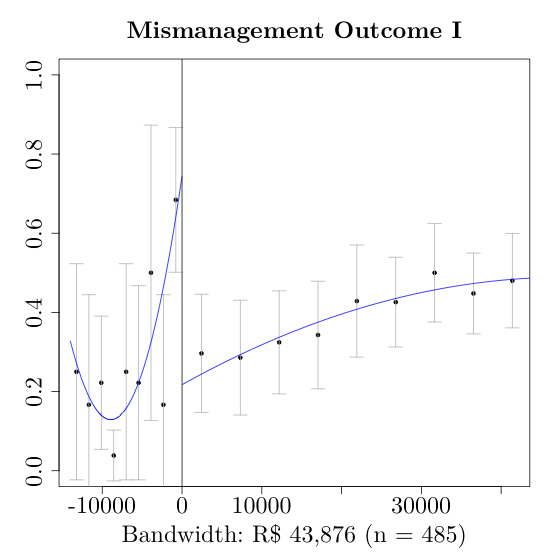
\includegraphics[scale = .265]{workscutoff1.png} & 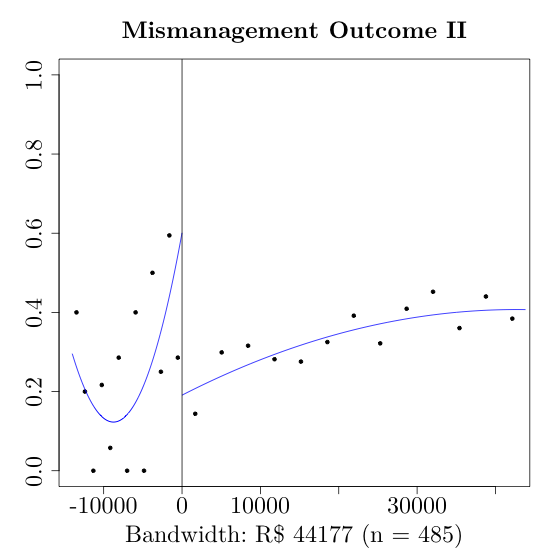
\includegraphics[scale = .265]{workscutoff2.png} & 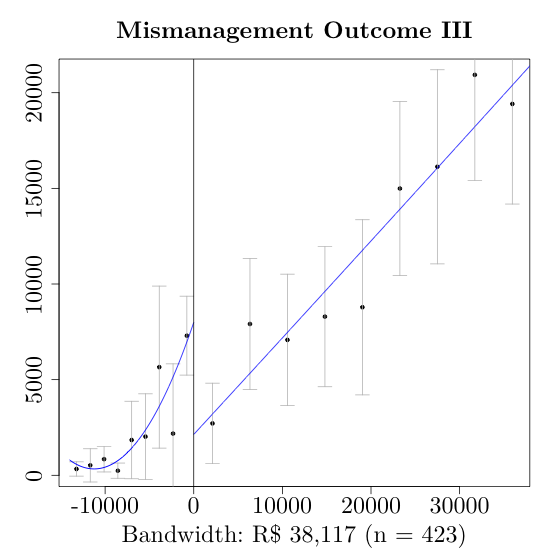
\includegraphics[scale = .265]{workscutoff3.png} \\
  \multicolumn{3}{p{\textwidth}}{\scriptsize Note: The three figures in figure \ref{fig:workscutoff1} report the minimum local causal effect of discretion (as a change in procurement rules from direct contracting to invitational bidding) on the three mismanagement outcomes. They plot the regression equations at the bandwidths specified in table \ref{tab:cctbandwidth} for mismanagement outcomes I through III when the federal transfer was used to procure goods or services used in public works. We also include 90\% confidence intervals in horizontal bars for each RD bin.}
  \end{tabular}
\end{figure}

Each graph uses the standard \citet{CalonicoOptimalDataDrivenRegression2015} bandwidths, a two-order polynomial fit for local estimating equations, and clustered-robust standard errors. We center the assignment variable (transfer amount) around zero, so all \emph{x} values are differences (in R\$) from the first cutoff for works at R\$15,000. We see statistically significant breaks in outcome means close to the cutoff for all three variables. For outcomes I and II, mismanagement increases at decreasing rates for observations further out to right, as the amount procured increases. The graphs for these two variables are similar, but they are complementary measures of performance. While outcome I summarizes the likelihood that any transfer sees mismanagement problems, outcome II looks at the share of all issues that are attributable to mismanagement \emph{conditional on finding any mismanagement problem}. Finally, the last outcome summarizes the amount potentially lost to corruption by multiplying outcome II and the transfer amount. The relatively large magnitude of this parameter (R\$4,611 in a R\$15,000 cutoff) means that the procurement legislation is preventing a large amount from being inefficiently applied.

\begin{figure}[!htbp]
  \caption{\label{fig:bandwidths} Discretion Point Estimates (Works SOs at Cutoff 1)}
  \centering
  \small
  \begin{tabular}{c}
  \emph{A: Mismanagement Binary} \\
  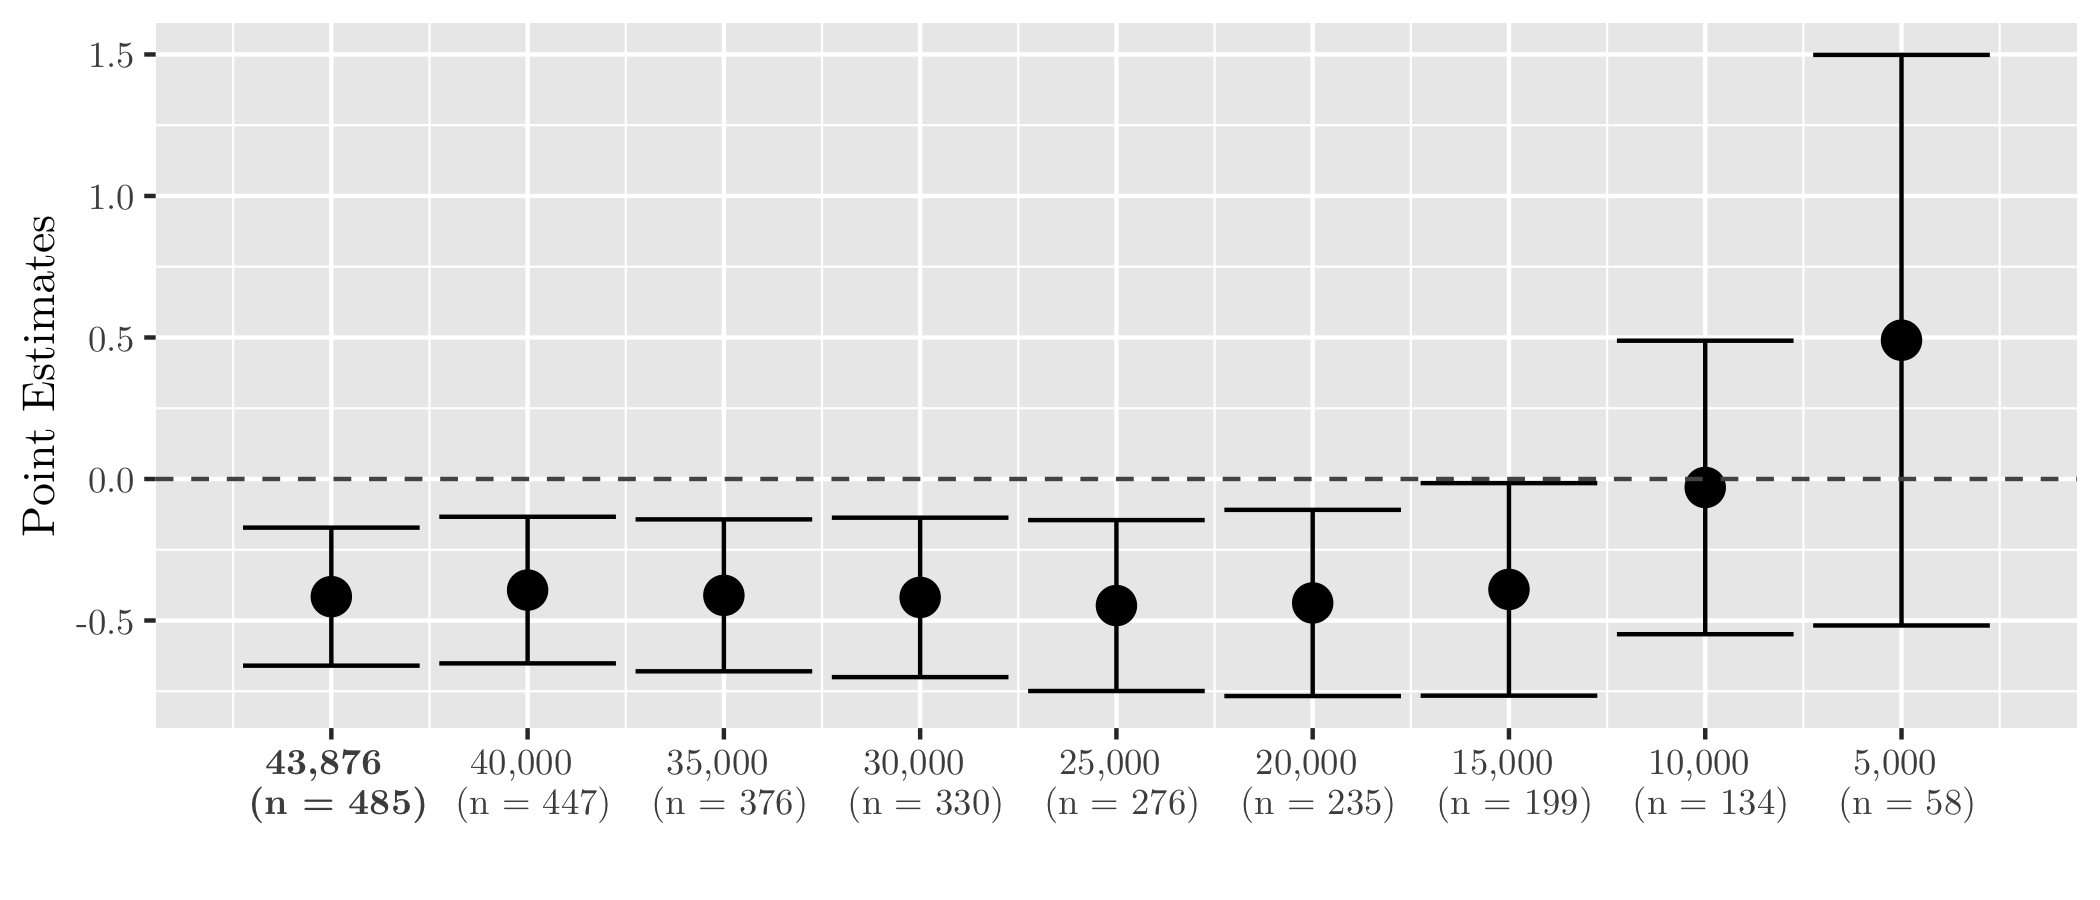
\includegraphics[scale = .14]{mismanagementplot1} \\
  \emph{B: Mismanagement Share} \\
  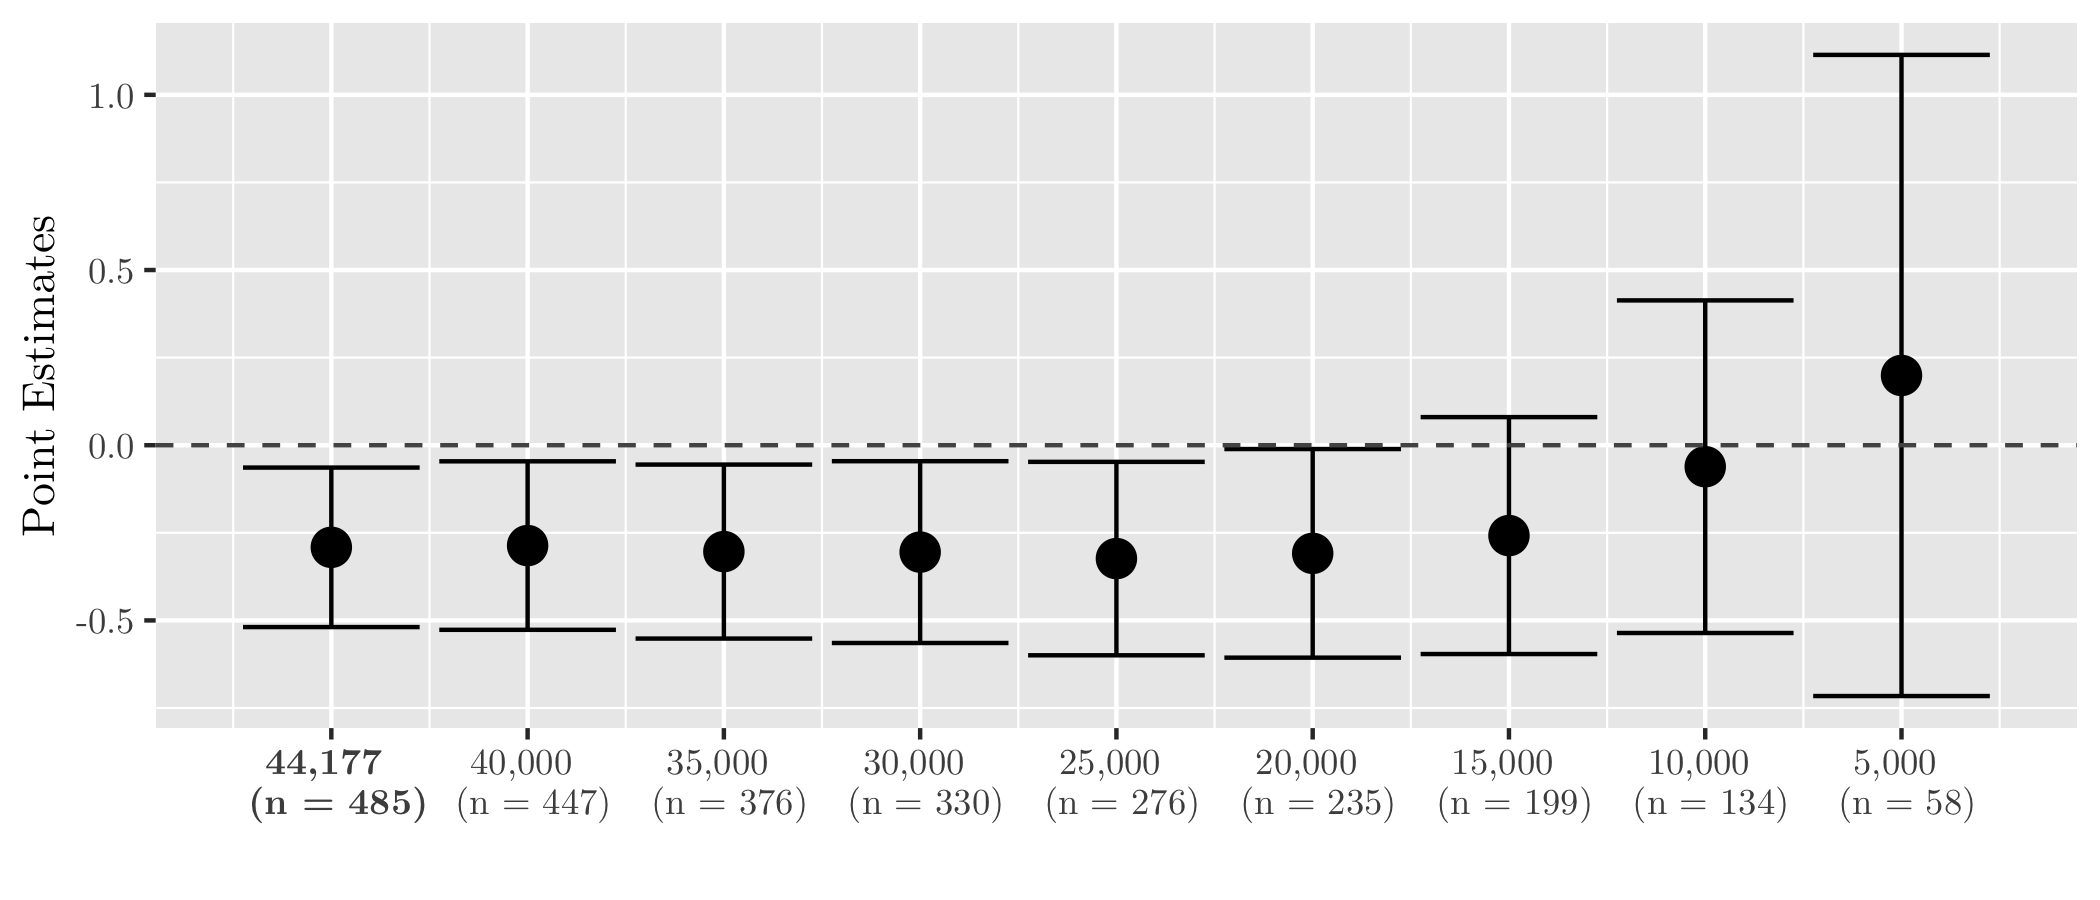
\includegraphics[scale = .14]{mismanagementplot2} \\
  \emph{C: Mismanagement Amount} \\
  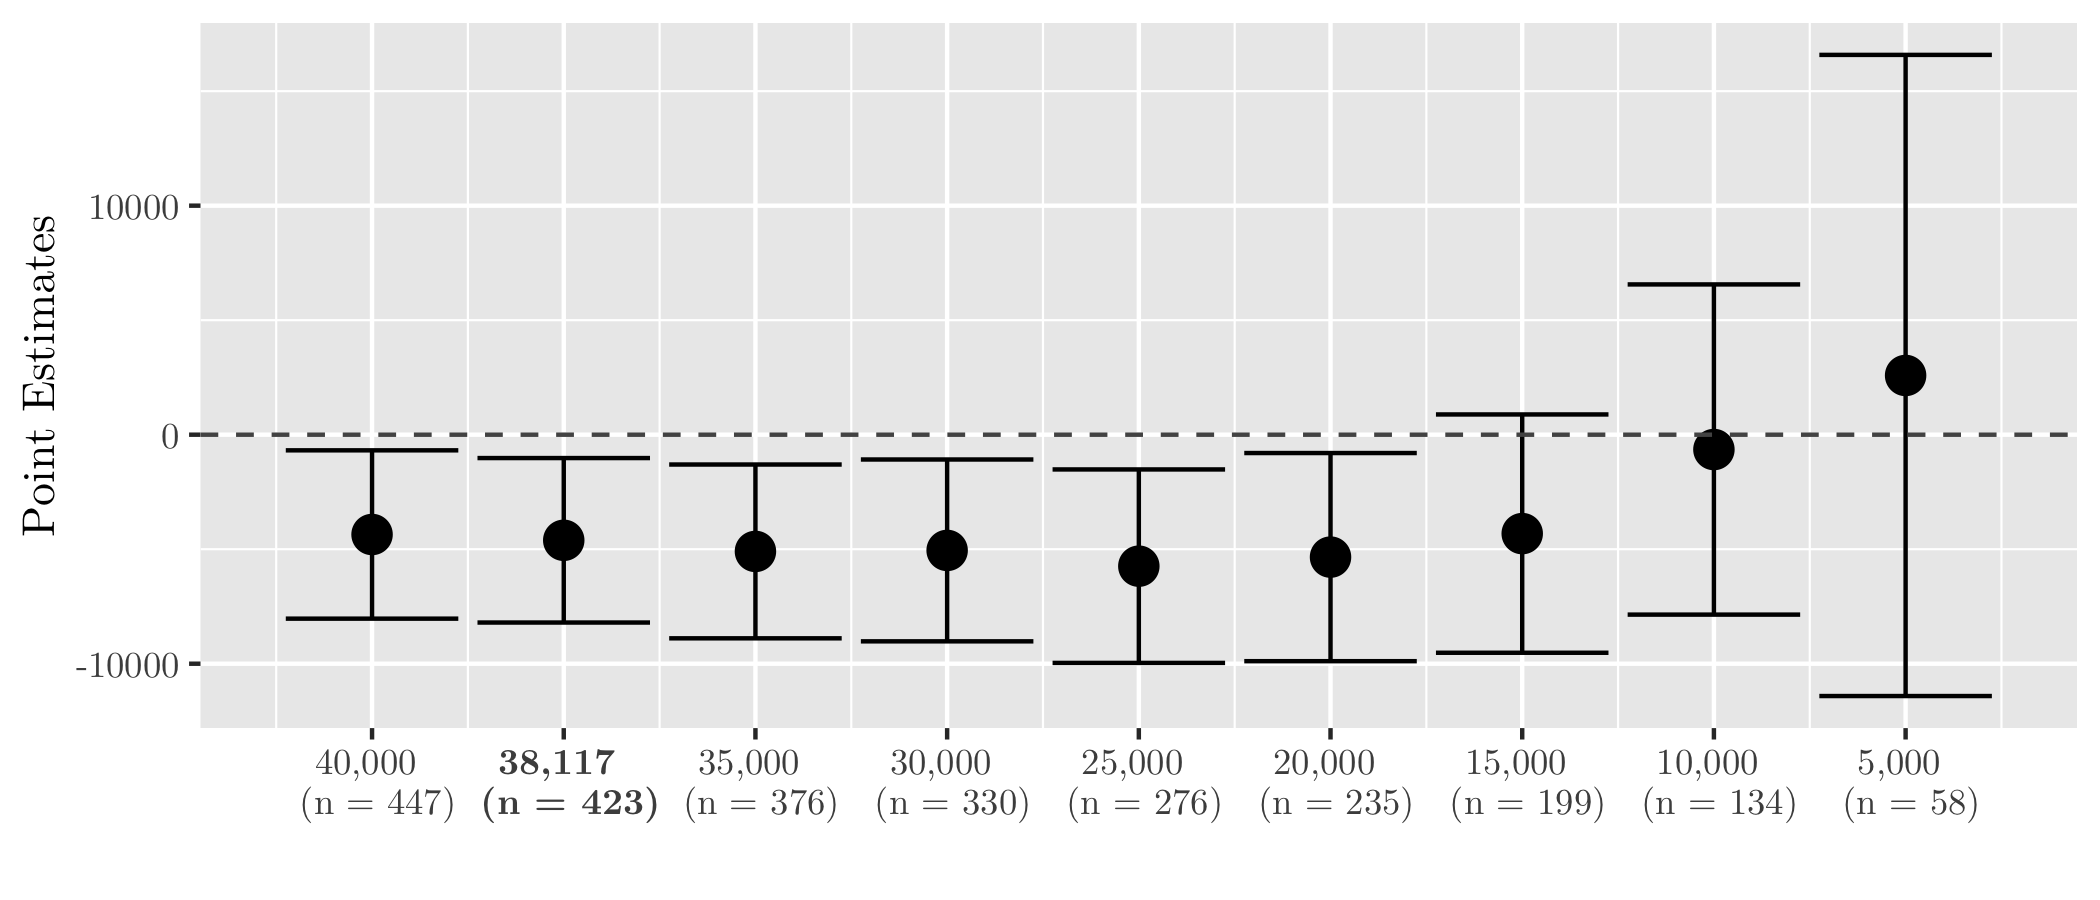
\includegraphics[scale = .14]{mismanagementplot3} \\
  \multicolumn{1}{p{.67\textwidth}}{\scriptsize Notes: These three graphs report the discretion point estimates and their 90\% confidence intervals for different bandwidths across works cutoff 1. The number of observations used in each local quadratic polynomial regressions is in parentheses across the horizontal axis. Confidence intervals overlapping the dashed lines show statistically insignificant parameters. \citet{CalonicoOptimalDataDrivenRegression2015} bandwidths are in bold.}
  \end{tabular}
\end{figure}

To further check the validity of our parameter estimates, we conduct a last test on the magnitude and significance of our discretion parameters for the works subsample at cutoff 1. In figure \ref{fig:bandwidths}, we use smaller bandwidths at which we calculate our lower-bounded LATE starting from the \citet{CalonicoOptimalDataDrivenRegression2015} and moving down until we reach R\$5,000 away from the cutoff on both sides. The point estimates are in the \emph{y}-axis while the \emph{x}-axis reports bandwidth and sample size. The point estimates are statistically different from zero for outcome I in seven out of nine bandwidths and six out of nine for outcomes II and III. The insignificant estimates at the smaller bandwidth are telling of the trade-off between significance and sample size in RD strategies. Were the samples larger, we would have seen the significant effect persist across all bandwidth sizes as standard errors would likely converge to that of significant parameters. Nevertheless, we propose two falsification tests in section \ref{subsec:discussion} which serve as additional evidence supporting the significant reduction of management problems when public officials have less freedom to allocate public resources (as measure by lower discretion in the procurement of goods and services for public works projects).

\subsection{Falsification Tests} \label{subsec:discussion}

In order to confirm the discretion effect reducing public works program management is not spurious nor due to random chance, we perform two additional tests on our sample of federal transfers.

The first test we conduct is mistakenly imposing the public works cutoff 1 on  purchases group observations. As a reminder, there are two types of procurement in Brazil: what we call \emph{purchases}, which consist of any purchase of goods and services, and \emph{public works}, which consist of purchases of goods and services to be used solely on public works projects. Since every public work requires procurement of any sort, the works group is a subsample of the overarching procurement of any good or service. If there is any significant effect of discretion at a falsified cutoff, then there is reason to believe the effect we identified is either spurious or random, therefore meaning that procurement restrictions have no improving effect on program management.

Similarly to figure \ref{fig:bandwidths}, we plot point estimates and 90\% confidence intervals for falsified cutoffs in figure \ref{fig:01falsification}. In these graphs, we are only using observations from the purchases subsample and running the exact same regressions as in sections \ref{sec:methodology} and \ref{sec:result} with two-order polynomial fits, clustered-robust standard errors, and the same varying bandwidths as in the works-only sample. Contrary to figure \ref{fig:bandwidths}, however, the optimal CCT bandwidth does not identify the largest possible sample, so we move from the same largest to smallest bandwidths as before.
\clearpage

\begin{figure}[!htbp]
  \caption{Discretion Point Estimates (Purchases SOs at Works Cutoff 1)}
  \label{fig:01falsification}
  \centering
  \small
  \begin{tabular}{c}
  \emph{A: Mismanagement Binary} \\
  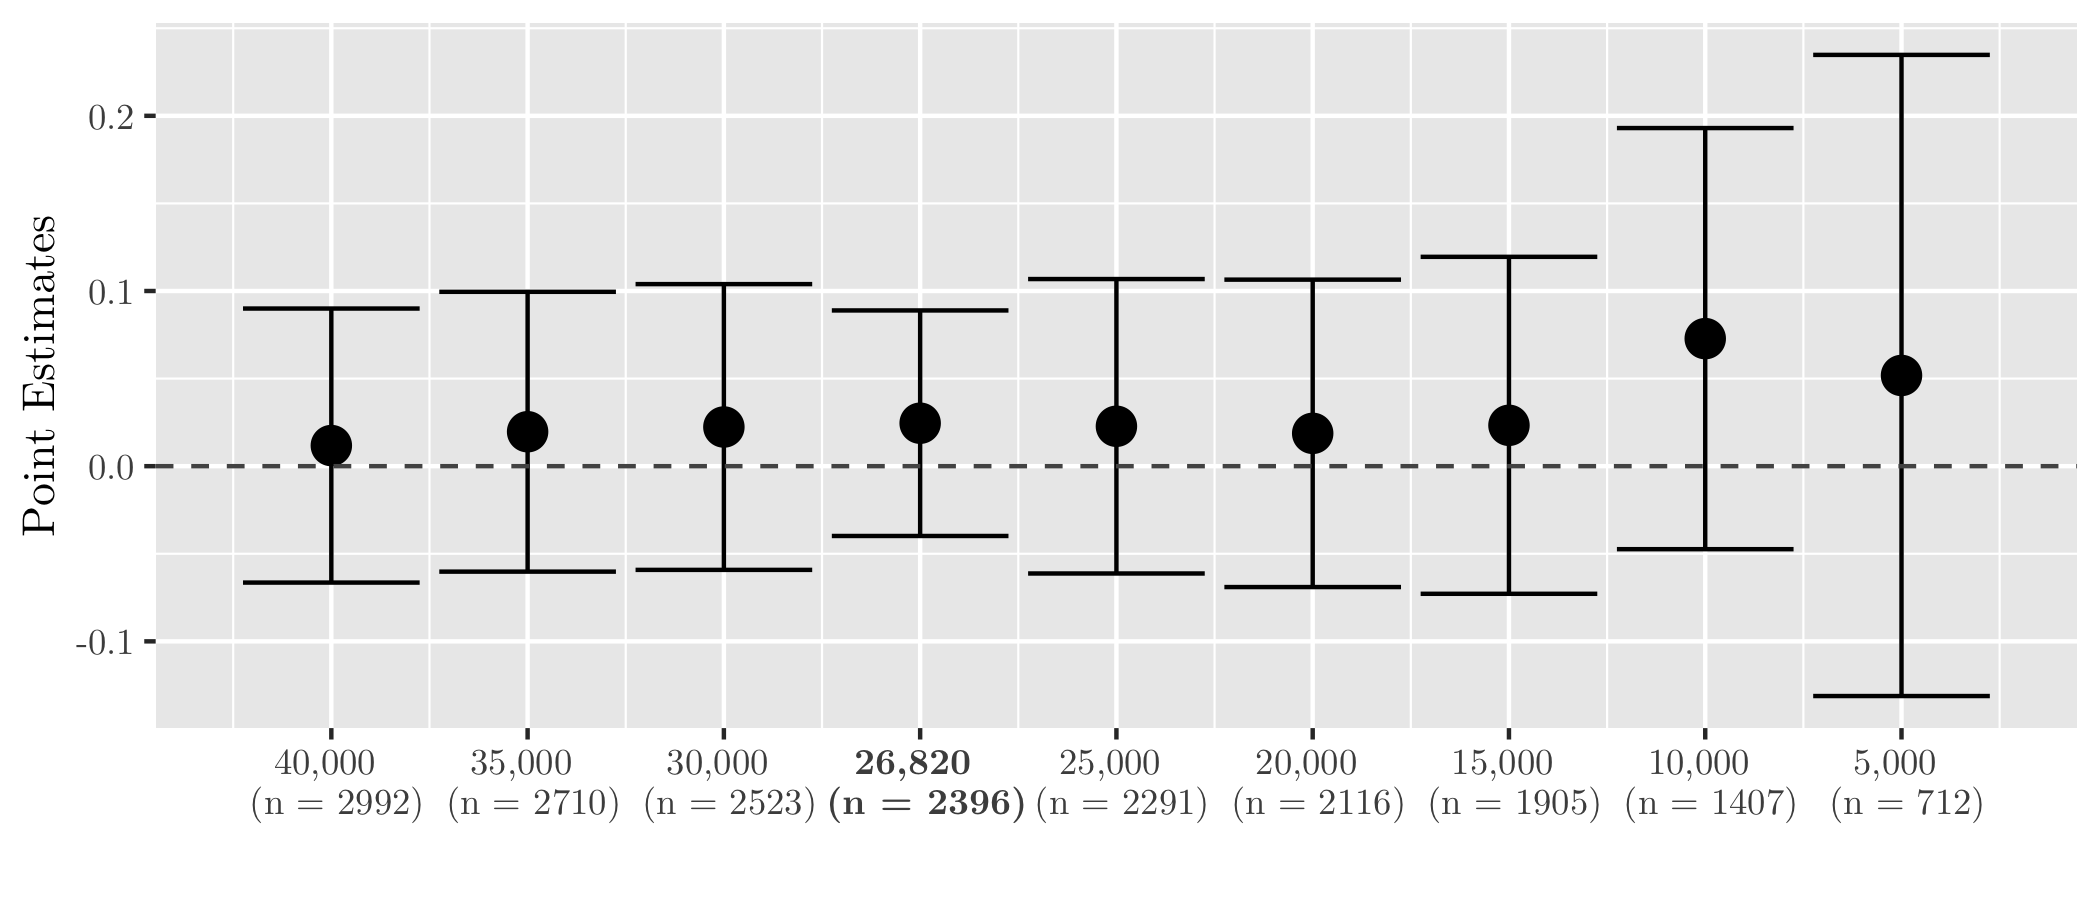
\includegraphics[scale = .14]{01falsificationplot1} \\
  \emph{B: Mismanagement Share} \\
  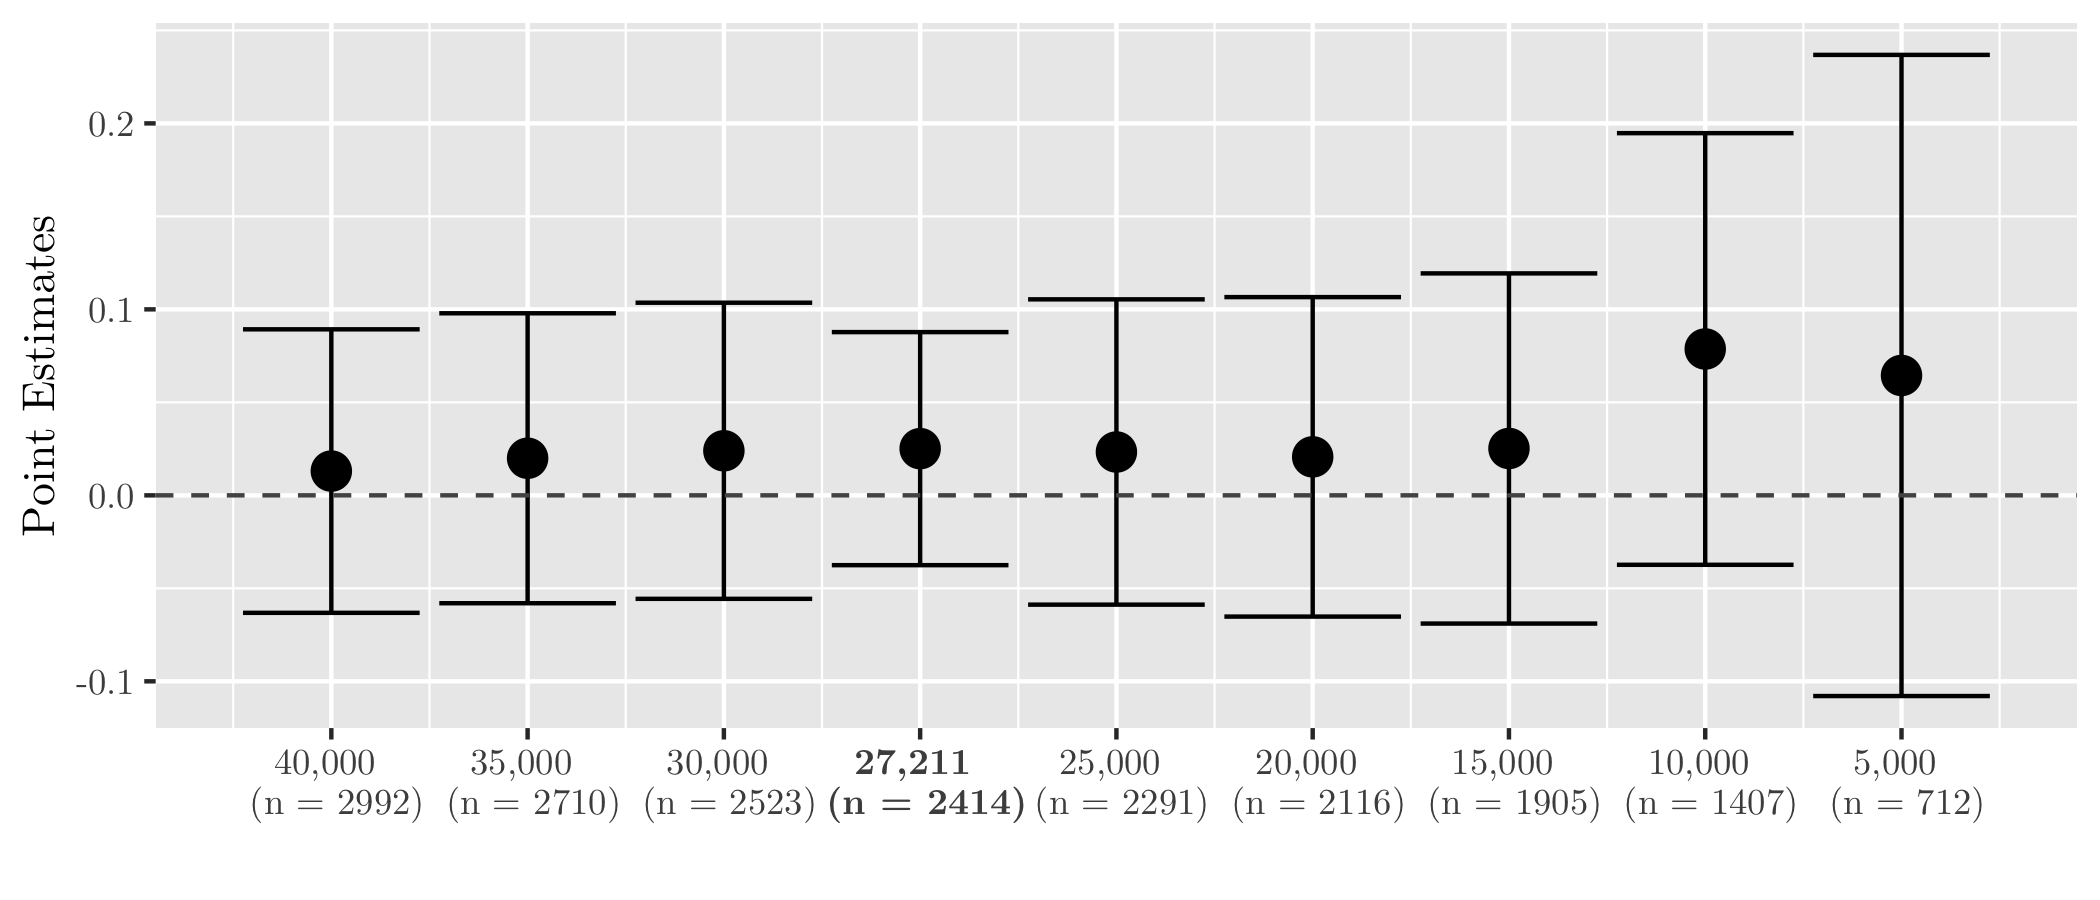
\includegraphics[scale = .14]{01falsificationplot2} \\
  \emph{C: Mismanagement Amount} \\
  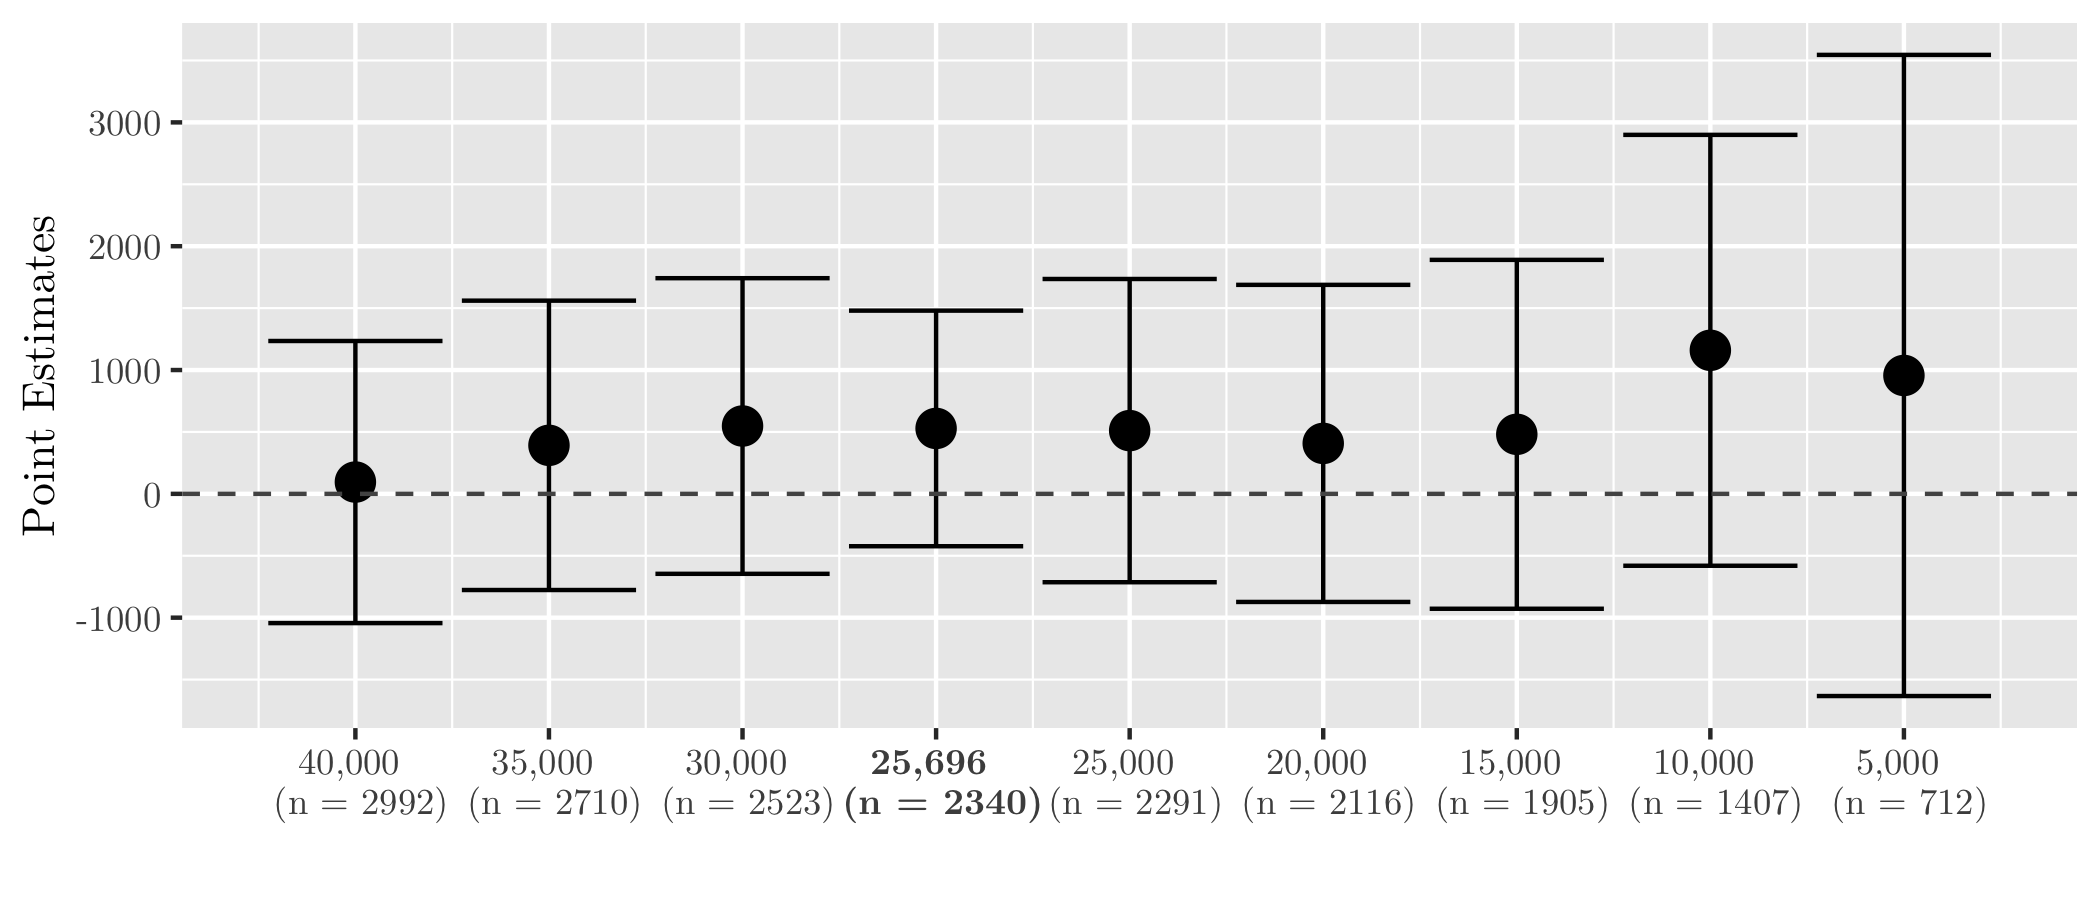
\includegraphics[scale = .14]{01falsificationplot3} \\
  \multicolumn{1}{p{.67\textwidth}}{\scriptsize Notes: These three graphs report the discretion point estimates and their 90\% confidence intervals for different bandwidths across works cutoff 1 \emph{using purchases SO as falsification data}. The number of observations used in each local quadratic polynomial regressions is in parentheses across the horizontal axis. Confidence intervals overlapping the dashed lines show statistically insignificant parameters. \citet{CalonicoOptimalDataDrivenRegression2015} bandwidths are in bold.}
  \end{tabular}
\end{figure}

There are no significant results across all figures at 90\% confidence intervals. Even with larger samples, there is no effect of the falsified cutoff on the likelihood of finding mismanagement, nor on the share of irregularities due to management problems, nor the amount potentially lost to resource misallocation. This is an important result supporting the evidence that the effect of discretion on mismanagement of public works projects is, in fact, non-random. Moreover, the point estimates are either close to zero or positive, which is opposite to the expected result in hypothesis 2 and confirmed in table \ref{tab:rdmc}.

An additional source of concern might be on the relationship between procurement legislation and program implementation. If procurement calls are carried out once for contracting the provision of goods and services, and their rules aim at preventing corruption, there is no direct link between imposing such rules and seeing better program implementation that occurs only after procurement has ended. We posited, however, that the work that goes into abiding by procurement rules also spread over better resource management practices, such as speedy procurement processes, that result in better program delivery. Quality and quantity requirements, delivery times, and the duration of contract for provision of goods and services are other factors included in procurement calls that can also improve public management. Therefore, there is a non-trivial benefit of restricting discretion on resource allocation.

The second falsification test investigates this relationship. In figure \ref{fig:02falsification}, we once again run the exact same regressions from sections \ref{sec:methodology} and \ref{sec:result} at varying bandwidths for the sample of \emph{non-procurement} federal transfers. This is a sample composed of 4,925 investigations (SOs) conducted by CGU auditors that were not identified as procurement because they met at least one of these conditions: (i) there was no textual description on the use of resources; (ii) there was no monetary amount reported by the auditor; (iii) the classification algorithm did not assign the investigation to any group. To further narrow down on non-procurement transfers, we exclude from this sample any investigation that could be matched to public works projects by grant description or by having works-related infractions as reported in audit reports (the two classification checks in appendix \ref{sec:appendixA}). The final non-procurement sample is composed of 2,493 investigations over the use federal resources for which auditors report the total value of transfer and for which there is not a single evidence of use in public works projects.\footnote{Non-procurement federal transfers are used for payment of personnel and new hires, covering budget shortfalls, for extension of procurement contracts after calls under Law 8,666/93 have been concluded, etc.}

A close look at figures \ref{fig:02falsification}.A through C reveals  no significant relationship between false cutoff 1 on mismanagement for the non-procurement sample (at the 90\% level). As we reduce the bandwidths around the false cutoff, all parameters remain indistinguishable from zero, though at smaller sample size we see much wider confidence intervals. Again with the case of public works true sample, more observations would help narrow down standard errors and potentially align parameter estimates along the results of larger bandwidths.
\clearpage

\begin{figure}[!htbp]
  \caption{Discretion Point Estimates (Non-Procurement SOs at Works Cutoff 1)}
  \label{fig:02falsification}
  \centering
  \small
  \begin{tabular}{c}
  \emph{A: Mismanagement Binary} \\
  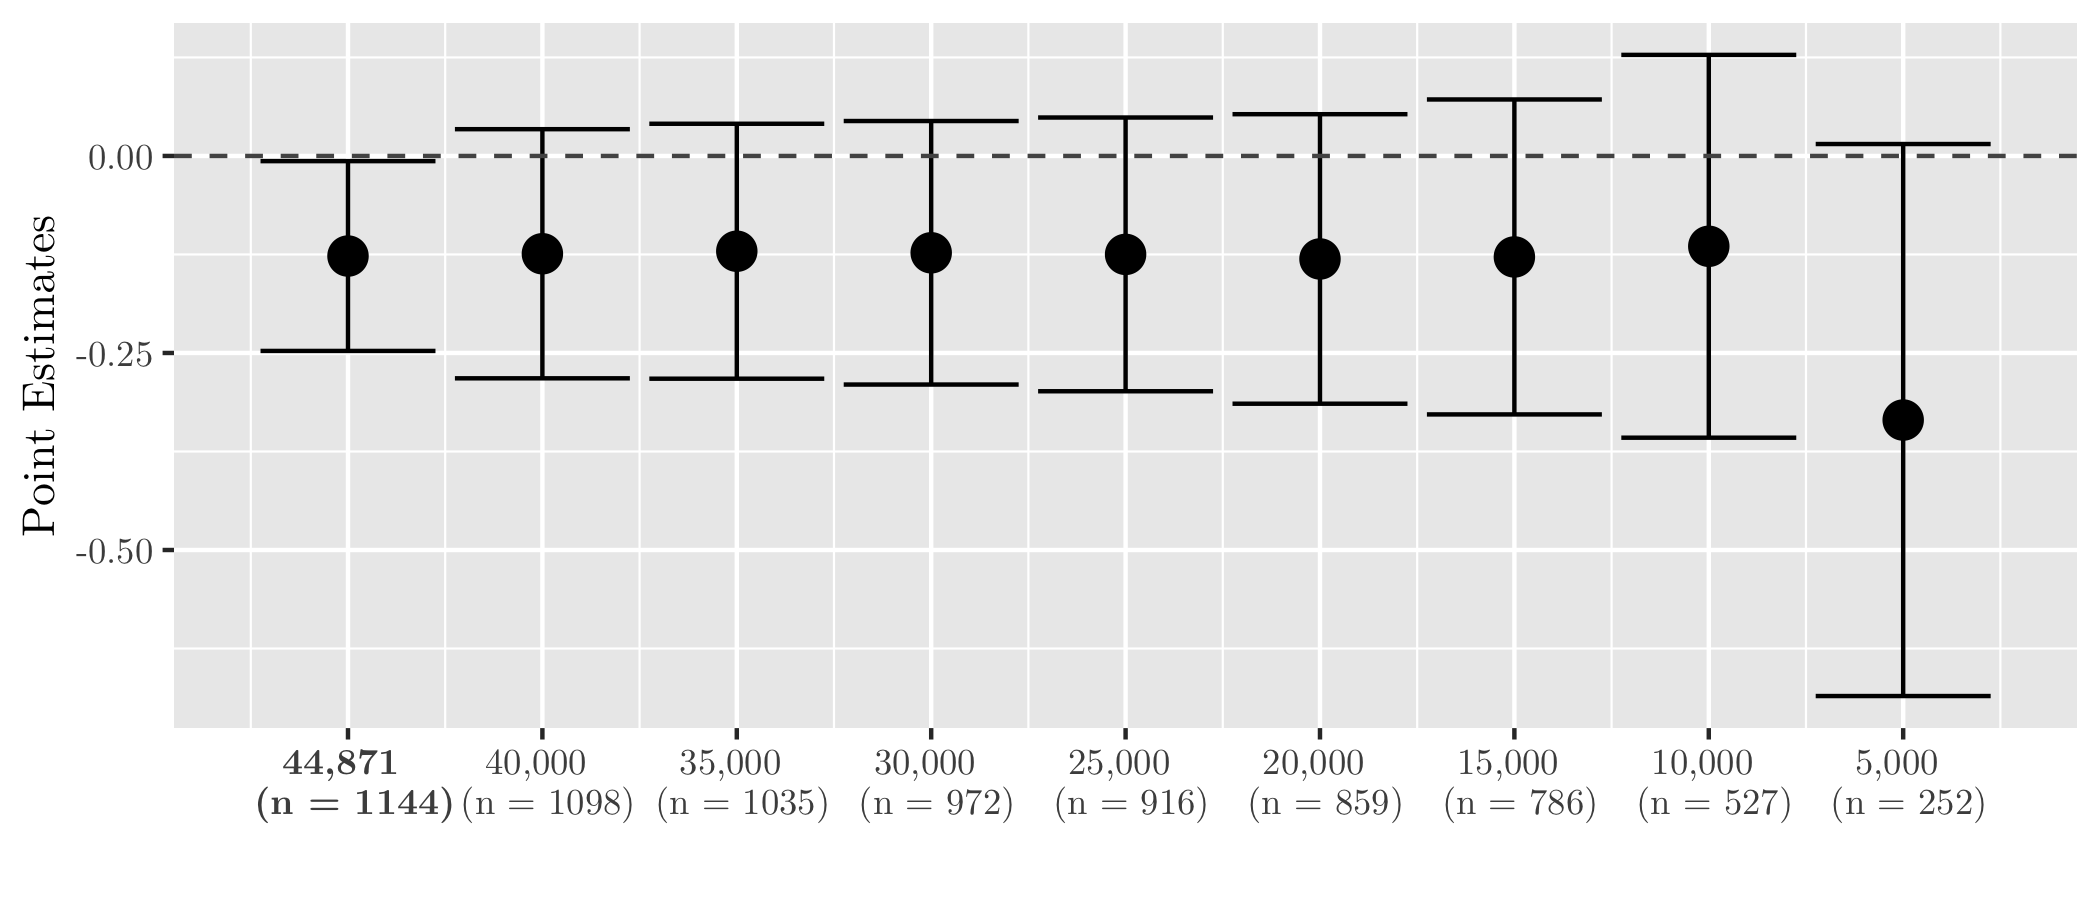
\includegraphics[scale = .14]{02falsificationplot1} \\
  \emph{B: Mismanagement Share} \\
  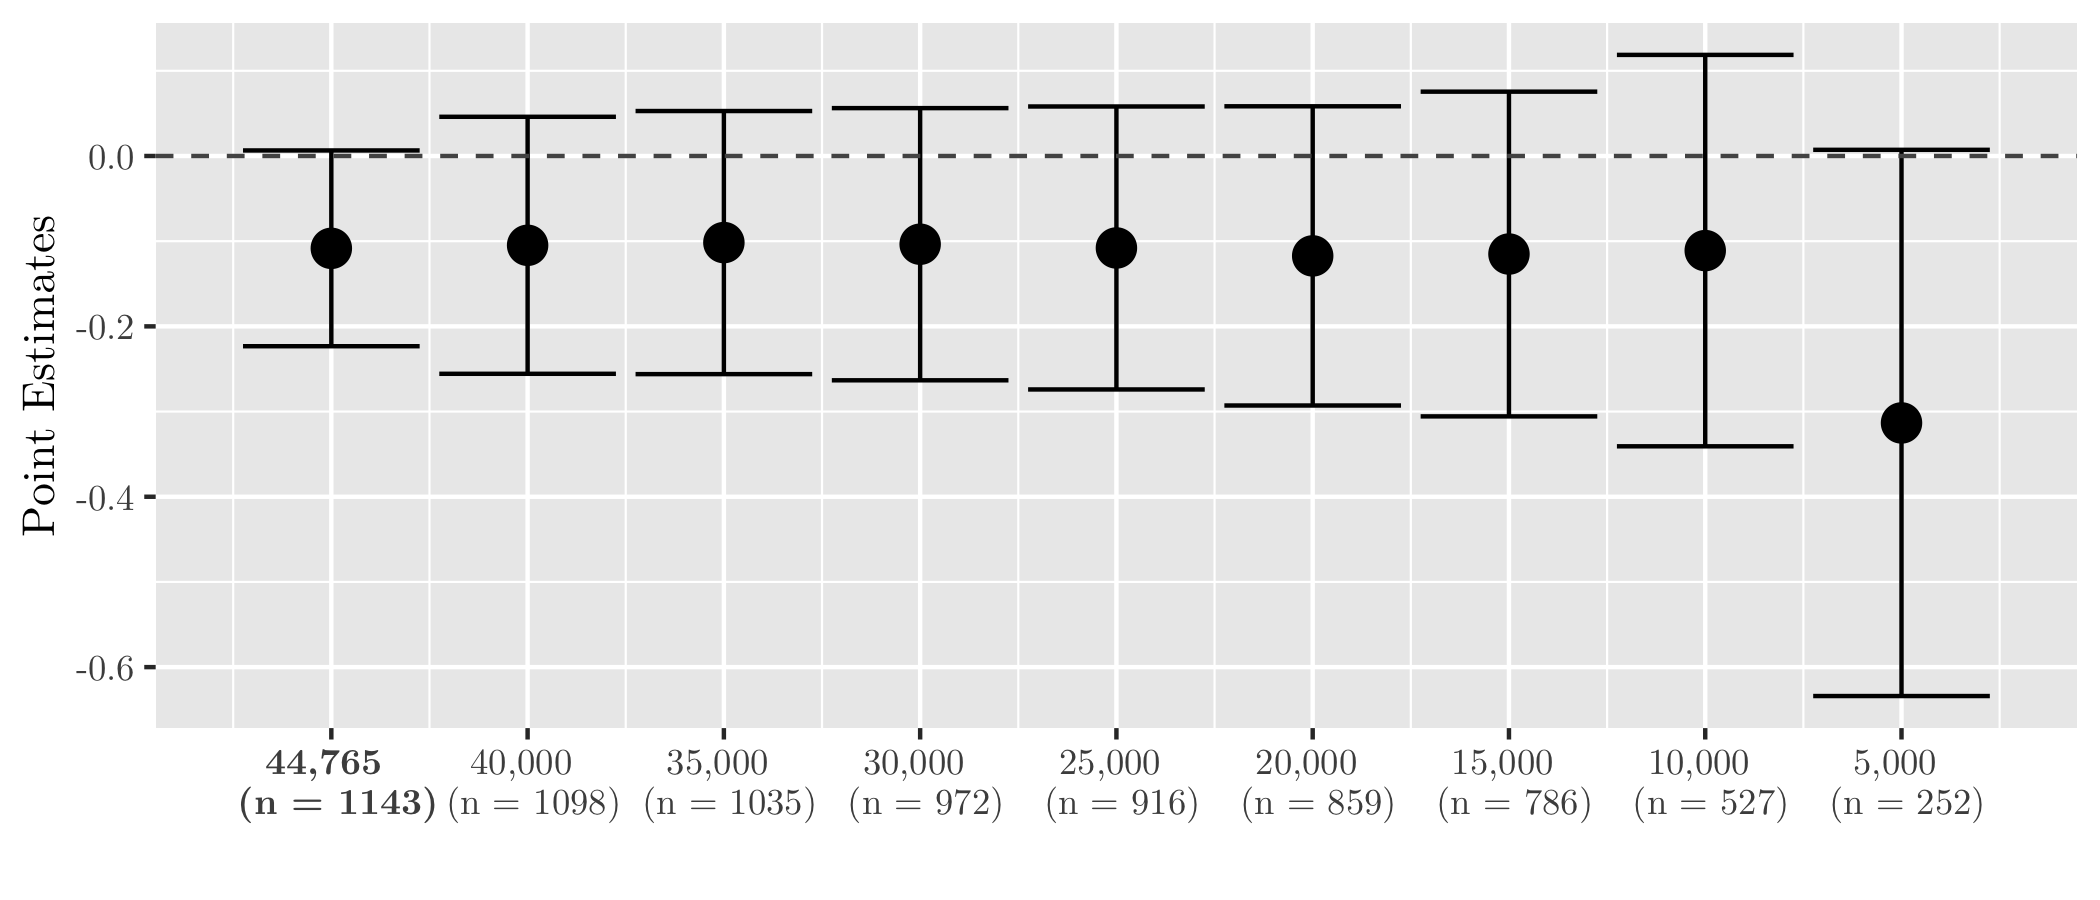
\includegraphics[scale = .14]{02falsificationplot2} \\
  \emph{C: Mismanagement Amount} \\
  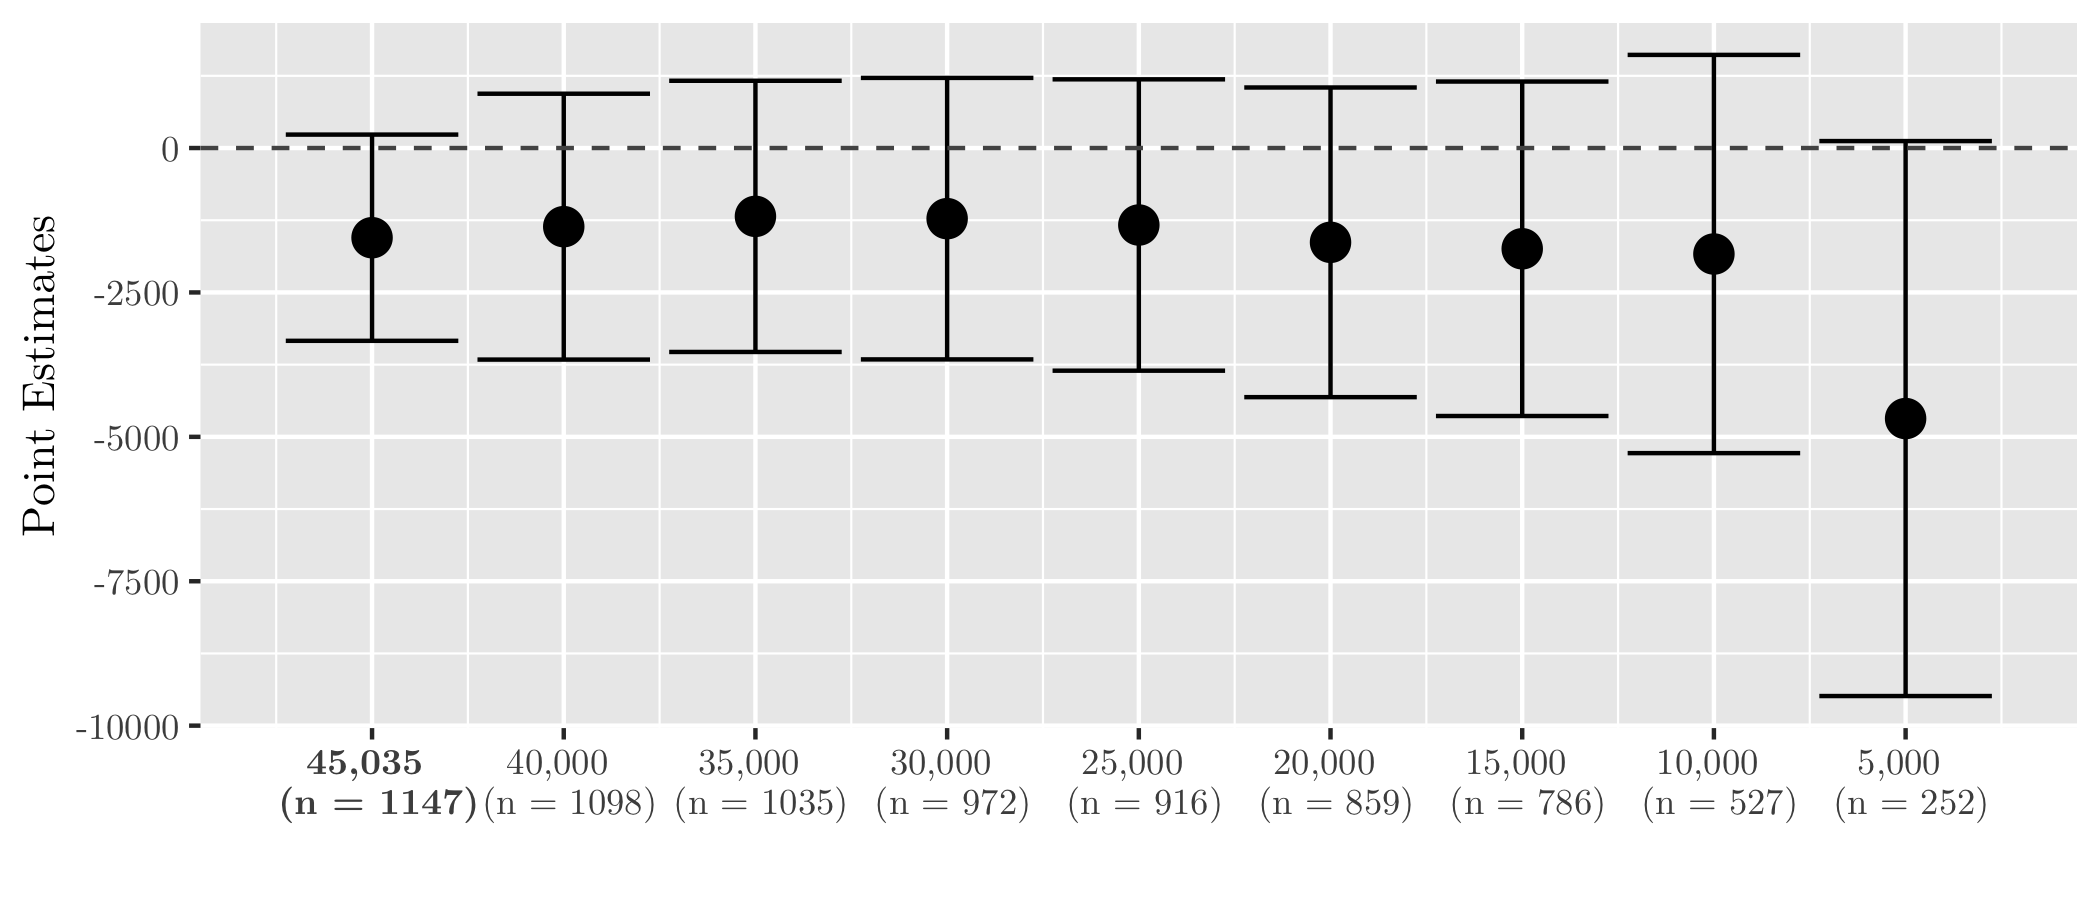
\includegraphics[scale = .14]{02falsificationplot3} \\
  \multicolumn{1}{p{.67\textwidth}}{\scriptsize Notes: These three graphs report the discretion point estimates and their 90\% confidence intervals for different bandwidths across works cutoff 1 \emph{using non-procurement SO as falsification data}. The number of observations used in each local quadratic polynomial regressions is in parentheses across the horizontal axis. Confidence intervals overlapping the dashed lines show statistically insignificant parameters. \citet{CalonicoOptimalDataDrivenRegression2015} bandwidths are in bold.}
  \end{tabular}
\end{figure}

\subsection{Interpretations of the Null Effect on Corruption} \label{subsec:nullcorruption}

In this section we return to our primary hypothesis and suggest possible interpretations for the null effect of discretion on corruption. It is naive to think that legislators knew nothing about corruption prevention and that Law 8,666/93 is entirely flawed. A more plausible explanation, however, is that corrupt behavior has changed over time while the procurement legislation has remained static. In this case, the law was appropriate under different corruption conditions than were present in our period of study (2004-2010).

The first potential interpretation is that public officials might have grown accustomed to procuring goods and services under the legal requirements and have thus been able to carry on practicing corruption while avoiding its detection. If this is the case, then we should not see differential levels of municipal corruption across time. We plot anecdotal data supporting this conclusion in table \ref{fig:01discussion}.

\begin{figure}[!htbp]
  \caption{Municipal Corruption Between 2004-2010}
  \label{fig:01discussion}
  \centering
  \small
  \begin{tabular}{c}
  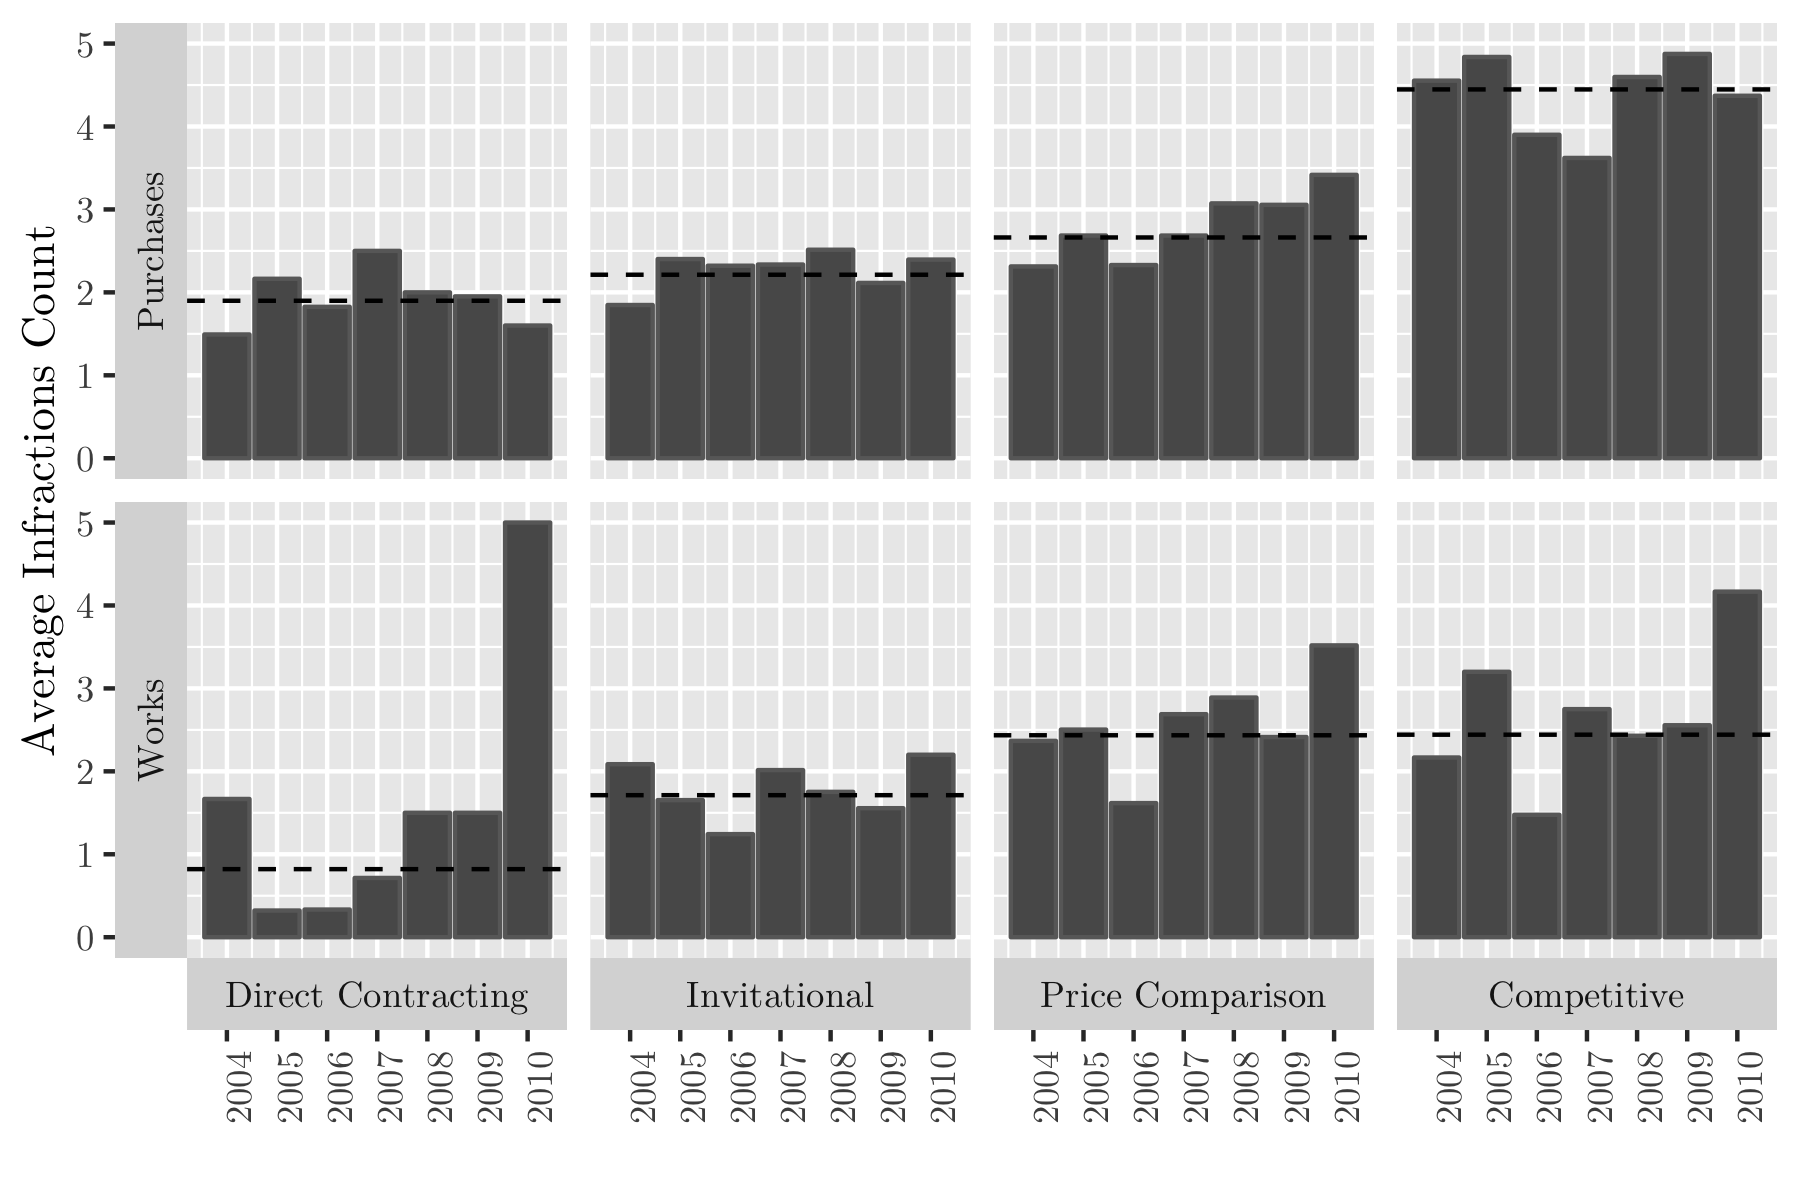
\includegraphics[scale = .14]{01discussionplot}
  \end{tabular}
\end{figure}

Municipal corruption levels are fairly stable over time. The average corruption share ranges between .18 to .21 of total infractions. Obviously, there are other things going on simultaneously besides learning the workaround procurement rule, but the relative stability of municipal corruption could also be a feature of the ease with which officials can sidestep rules if they want to engage in corruption. Moreover, the burden for corruption falls more heavily on mayors \citep{FinanGovernmentAuditsReduce2018} than on their lower level staff.

Another explanation to the null effect is the decreasing purchasing power of public resources in the presence of inflation. Since the cutoffs across categories remain constant over the period under analysis, inflation reduces the quantity of goods and services any single procurement call can contract, thus turning small procurement amounts (regulated by lower categories of Law 8,666/93) meaningless in terms of their complexity or the corruption opportunity they create. This means that compliance at lower categories of the procurement law might be easier due to the relative simplicity, lower quality, or smaller quantity of the items being procured. The propose checking this explanation by looking at the average number of infractions (both in corruption and management) across time, procurement type, and category. We present the results of this tabulation in \ref{fig:02discussion}, where we see the average number of infractions per investigation on the \emph{y}-axis, and the year of investigation on the \emph{x}-axis. We further split the results by type of procurement (public purchases or works) and category (direct contracting, invitational bidding, price comparison bidding, and competitive bidding). Thus, each quadrant summarizes the average number of infractions per year, procurement type, and category. The dashed black lines are the average number of infractions across type and category and removes the variation at the time dimension.

\begin{figure}[!htbp]
  \caption{Average Infraction Count Per Year, Procurement Type, and Category}
  \label{fig:02discussion}
  \centering
  \small
  \begin{tabular}{c}
  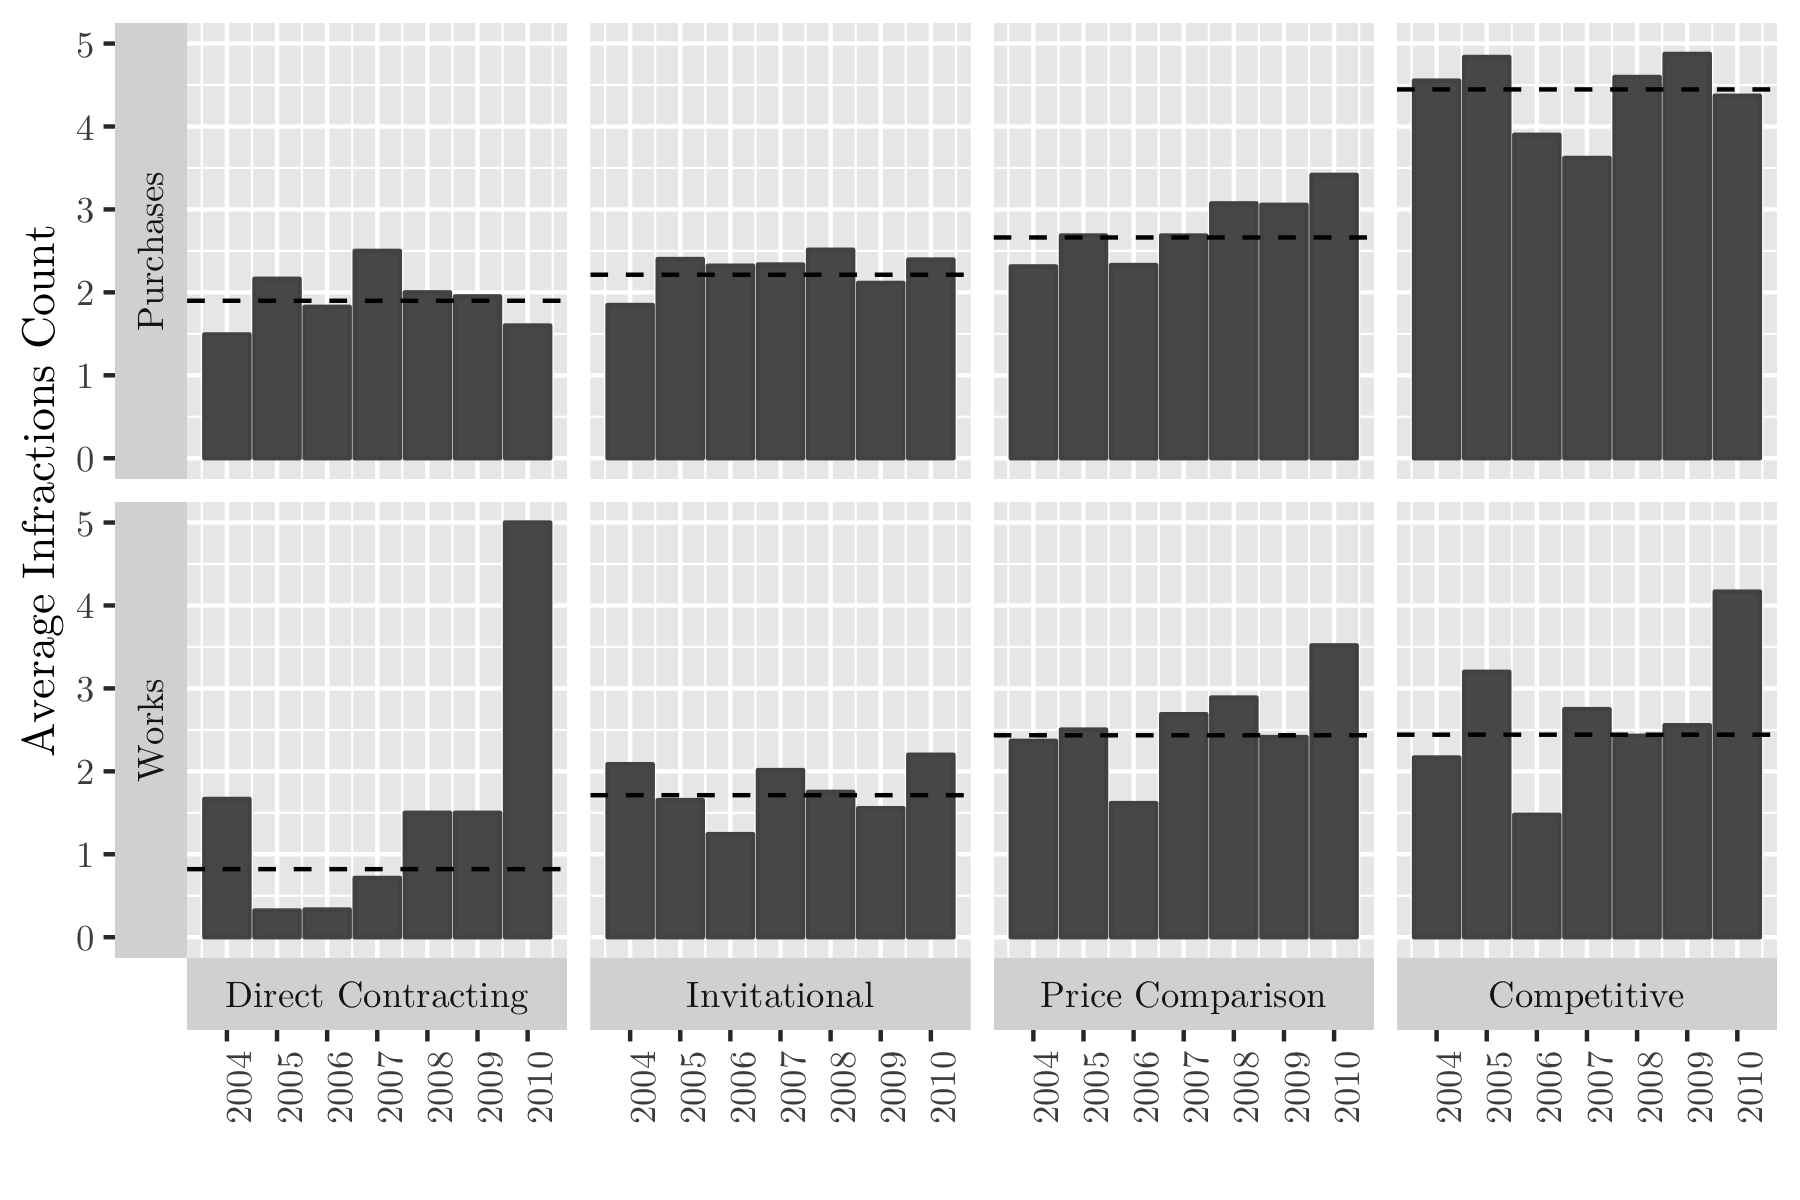
\includegraphics[scale = .2]{02discussionplot}
  \end{tabular}
\end{figure}

Across both types of procurement, we see the average number of infractions increase as we move up procurement categories (shown by the level of the dashed black lines read from left to right). Though not conclusive, this is suggestive of decreasing compliance with program specification and procurement rules. For the purchases group, the top four quadrants, we see relative stability of the average number of infractions which, read along figure \ref{fig:01discussion} on the share of corruption issues, indicates little variation in the number of management problems as well. For the works group, in the bottom four graphs, we see 2006 and 2010 as outline years for lower and higher averages, respectively. The jump in infractions between quadrants one and two, representing direct contracting and invitational bidding, are consistent with the management effect of discretion in section \ref{sec:result}: since there are no significant changes in corruption at this cutoff, most of the change in averages (from .9 to 1.6) must come from program management infractions.

These are but two interpretations of the null effect on corruption and we do not aim at exhausting the alternative explanations for such unexpected effect. We suggest these puzzles as avenues for future research on the effect of discretion on performance.

\subsection{Cost-Benefit Analysis} \label{subsec:cba}

So far, we have focused on testing our hypotheses and uncovering potential confounding effects of discretion. We now move on to discuss the welfare effects of law 8,666/93, which should serve as a transparent metric to support or reject the procurement law.

The only significant, beneficial effect is the reduction in mismanagement for the public works sample at the change in rules from direct contracting to invitational bidding. The costs, however, are all other corruption and mismanagement problems not prevented at the equivalent cutoffs. We conduct a back-of-the-envelope cost-benefit analysis (CBA) in table \ref{tab:welfare}.

% latex table generated in R 3.5.1 by xtable 1.8-2 package
% Fri Aug 24 13:10:19 2018
\begin{table}[!htbp]
  \centering
  \caption{\label{tab:welfare}Welfare Effects from Discretion at Cutoff 1}
  \scriptsize
  \begin{tabular}{lrrrr}
  \hline

  \hline
  \emph{Cost}                                    & Type      & Avg. Loss (in R\$) & \# Obs. & Total (in R\$) \T \B \\
  \hline
  Corruption                                     & Purchases & 2,491              & 1,934   & 4,818,570  \T \B \\
  Mismanagement                                  & Purchases & 10,659             & 1,924   & 20,508,793 \T \B \\
  Corruption                                     & Works     & 2,871              & 314     & 901,789    \T \B \\
  Mismanagement                                  & Works     & 10,529             & 423     & 4,454,134  \T \B \\
  \hline
  \multicolumn{4}{r}{\emph{Total Cost $(A)$}}    & 30,683,288 \T \B \\
  \emph{Benefits}                                &  &  &  &  \\
  \hline
  Works                                          & Mismanagement & -4,611 & 423 & -1,950,453 \T \B \\
  \hline
  \multicolumn{4}{r}{\emph{Total Benefit $(B)$}} & -1,950,453 \T \B \\
  \emph{Welfare Effect}                          &  &  &  &  \\
  \hline
  $A-B$                        & \multicolumn{3}{r}{\emph{Total Cost (in R\$) in the absence of Benefit}} & 32,633,741 \T \B \\
  $100 \times B/(A-B)$         & \multicolumn{3}{r}{\emph{\% Cost Reduction}}                             & 5.98       \T \B \\
  $A_{works} - B$              & \multicolumn{3}{r}{\emph{Works Cost (in R\$) in the absence of Benefit}} & 7,306,377  \T \B \\
  $100 \times B/(A_{works}-B)$ & \multicolumn{3}{r}{\emph{\% Works Cost Reduction}}                       & 26.69      \T \B \\
  \hline

  \hline
  \end{tabular}

\end{table}


In the top part of the table, we calculate the costs of law 8,666/93 as the total misplaced amount not prevented by invitational bidding contracting rules. These costs come from both procurement types, public purchases and works, and outcomes, corruption and mismanagement. In column three, average loss in R\$, we include the average amount misplaced due to either problem for all observations within the CCT bandwidth around cutoff 1. Since our parameters are lower-bounded LATE, they only constitute causal effects at the vicinity of the procurement rule discontinuity, thus the focus on these subsamples. We multiple each average cost by the number of observations and add them up to a total cost (A) over R\$30M (last row of top part).

The total benefit, on the other hand, comes from the amount that would have been misplaced had law 8,666/93 not been in effect. On column three, in the middle part of the table, the average loss prevented is the LATE parameter at works cutoff 1 for mismanagement outcome III, which calculates the amount potentially lost by multiplying the share of mismanagement issues times the transfer amount. $(B)$ is the total misallocation prevented, approximately R\$2M.

Finally, we report welfare effects at the bottom part of the table. We calculate both misallocation prevention in absolute (R\$) and relative (\%) terms. Total cost of misallocation would be approximately R\$32.5M and the works-only cost would be R\$7.7M (compared to R\$4.4M in the absence of the law). Moreover, the discretion change reduces total cost by 5.98\% and 26.69\%, respectively, for total cost and public works projects. Although this is a substantial reduction in misplaced funds, R\$30M still remain unaccounted for, and its misallocation could have been prevented had the procurement legislation been adapted over time. Citizens and legislators should compare this potential recovery to overall municipal budgets in order to figure out whether law 8,666/93 should be kept.


\section{Conclusion} \label{sec:conclusion}

In this paper, we looked at the effect of discretion in public spending on government performance. We operationalize this relationship by exploring the Brazilian procurement law 8,666/93, which determines rules that should be followed at all government level and branches when procuring goods and services. Our observations are investigations conducted by CGU's random audit program between 2004 and 2010, from which we can create objective measures of corruption and mismanagement of public resources. We infer procurement type using a text analysis algorithm developed by one of the authors, described in the appendix, to match each investigation to procurement types and categories established by Law 8,666/93. Besides contributing to the literature by exploring discretion as determinant of government performance, we also investigate whether performance is associated with the overall procurement amount and local municipal corruption.

We cannot confirm that discretion reduces corruption. Using our preferred RD identification strategy, we find no significant effect of discretion on corruption, regardless of whether the procurement call was motivated by public works projects or any other provision of goods and services. This results has a direct, and important, policy implication regarding the support for the Brazil procurement law. In the sample framework outlined in section \ref{subsec:hypotheses}, legislators and citizens would both weakly support legislation that does not deliver on its promise of reducing corruption.

Some explanations emerge for the non-significant effect on corruption. The strongest interpretation we suggest is that the inflation-unadjusted amounts determining procurement rules have become meaningless over time. Procurement compliance for items of lower amount might just be simpler than at higher contract values. In fact, figure \ref{fig:02discussion} shows that the average number of infractions is increasing both across time and procurement categority, suggesting that non-compliance infractions are less frequent as the purchasing-power of procurement calls decreases. Additionally, \citet{FinanGovernmentAuditsReduce2018} show that the likelihood of punishment for corruption is low and, if at all, fall more heavily on mayors than on lower-level officials. If this is the case, then officials have relatively more incentives for non-compliance and are likely to keep the same level of corruption regardless of rules imposing less discretion (anecdotal evidence in figure \ref{fig:01discussion}).

The discretion effect on mismanagement is moderate at best. We find no effect for the general procurement group (\emph{purchases}) but find a consistent effect on reducing program management problems when moving from directly contracting with private suppliers to invitational bidding when the city government contracts goods and services for public works projects. The likelihood of finding any mismanagement problem decreases by 41.6 percentage points. Conditional on finding any issue, the share of program management infractions falls by 29.1 when implementing stricter rules and the amount potentially misplaced reduces by R\$4,611. Though our results are concentrated in one cutoff and for one type of procurement, they are important initial evidence disentangling the effect of discretion from broader measures such a political decentralization and devolution of funds. Since our estimates are lower-bounded LATE, there still remains a large field of research for identifying precise discretion effects across the entire distribution of public spending decisions.

To check these results, we suggest two falsification tests: running the same regressions that yielded significant parameters on falsified datasets for which there should be no effect. We used the purchases and the non-procurement samples to confirm (i) that the effect is exclusive to public works procurement and (ii) that procurement is indeed relevant for government performance. There are no significant effects on mismanagement at the falsified cutoffs, regardless of the data we use.

Lastly, we provide a rough estimate of the costs and benefits of the procurement legislation in Brazil for a transparent metric with which to decide whether discretion restrictions should be kept or not. Though the legislation reduces the total amount of missing funds by 5.98\%, there are still R\$30M missing -- equivalent to six times the yearly average funds transferred from the federal government to municipalities in the period under analysis. Discretion restrictions, all included, might not be the best way to improve government performance.

\clearpage

\setlength\bibsep{0pt}
\bibliographystyle{apalike}
\bibliography{/Users/aassumpcao/library.bib}

\clearpage

% \singlespacing

% \section*{Tables} \label{sec:tab}

% \clearpage

% \section*{Figures} \label{sec:fig}

%\begin{figure}[hp]
%  \centering
%  \includegraphics[width=.6\textwidth]{../fig/placeholder.pdf}
%  \caption{Placeholder}
%  \label{fig:placeholder}
%\end{figure}


\clearpage

\appendix

\section{Appendix: Service Order Classification} \label{sec:appendixA}

Service orders issued by CGU investigated various uses of public resources in addition to procurement, e.g.~for staff compensation, for school activities, or for community monitoring of public policies. The discretion measure proposed in this paper, however, is only applicable to uses of public resources that required the procurement of goods and services under Law 8,666/93. Therefore, the ideal dataset for this study would contain, for each federal transfer, the attached procurement call informing dates, goods/services procured, global contract value, who was awarded the contract, and so on. Unfortunately, there is no organized, public database of municipal contracting processes. In CGU's reports, the reporting of procurement calls is implicit, via descriptions of investigations or violations to Law 8,666/93. Thus, we isolate service orders for which there was any procurement of goods/services involved from the rest by implementing a classification system based on the information retrieval literature.

The system uses each service order's description to identify if it is procurement-related. In these descriptions, CGU auditors report the purpose of their investigation, e.g.~whether they are looking into drug purchases, whether the municipality has used the funds within designated program goals, or whether primary school teachers were hired for the implementation of a school program. Using these textual descriptions as bag-of-words models, we implement a method similar to that of \citet{HopkinsMethodAutomatedNonparametric2009}: we stem and combine procurement-related keywords to form patterns to be searched for in the description of each investigation conducted by CGU. There are two broad types of procurement in Law 8,666/93: (i) ordinary procurement of goods and services, which we call \emph{purchases}; and (ii) procurement of goods and services used for public works, which we call \emph{works}. There are different search patterns for each group.

An example is useful for understanding our classification process. Unigram ``aquisição'' (\emph{acquisition} in English) is stemmed to ``aquisi'' to form a search pattern for the \emph{purchases}-type procurement; unigrams ``adequação'' and ``habitacional'' (roughly translated as \emph{housing adequacy}) are stemmed and combined to form ``adequa(.)*habitac'' search pattern for \emph{works}-type procurement. The use of bigrams and regular expressions, such as in the pattern above, picks up variations in main keywords as well as coding mistakes due to, for instance, multiple whitespace between the two unigrams or due to coding Portuguese special characters (``adequação'' vs. ``adequacao'').

\begin{table}[!htbp]
  \caption{\label{tab:searchterms} Procurement Search Terms (in regular expression format)}
  \centering
  \scriptsize
  \begin{tabular}{l p{.85\textwidth}}
  \hline

  \hline
  Type & Search Terms \T \B \\
  \hline
  Purchases & ``aquisi'' ``execu'' ``equipame'' ``ve{[}íi{]}culo'' ``despesa'' ``aplica{[}çc{]}'' ``medicamento(.)*peaf'' ``compra'' ``recurso(.)*financ'' ``unidade(.)*m{[}óo{]}ve(.)*sa{[}úu{]}de'' ``pnate'' ``transporte(.)*escola'' ``desenv(.)*ensino'' ``kit'' ``siafi'' ``implementa{[}çc{]}'' ``adquir'' ``pme(.)*2004'' ``aparelhamento'' \T \B \\
  \hline
  Works & ``co(ns\textbar{}sn)tru'' ``obra'' ``implant'' ``infra(.)*estrut'' ``amplia'' ``abasteci(.)*d(.)*{[}áa{]}gua'' ``reforma'' ``(melhoria\textbar{}adequa)+(.)*(f{[}íi{]}sica\textbar{}escolar\textbar{}habitac\textbar{}sanit{[}áa{]}ria)+'' ``esgot'' ``adutora\textbar{}dessaliniz\textbar{}reservat{[}óo{]}'' ``sanit{[}áa{]}ri{[}ao{]}'' ``poço'' ``aperfei{[}çc{]}oa'' ``saneamento'' ``res{[}íi{]}duo(.)*s{[}óo{]}lido'' ``conclus{[}ãa{]}o'' \T \B \\
  \hline

  \hline
  \end{tabular}
\end{table}

The final list contains 19 \emph{n}-grams for identification of purchases and 17 \emph{n}-grams for works.\footnote{One of these keywords in the works search pattern is an ``exclusion keyword,'' which removes service orders that contain the ``exclusion keyword'' in their description from the sample identified by the other 16 \emph{n}-grams.} When any of these words is found, we include the service order into the purchases or the works group. Since all public works projects procure goods and services but not all public purchases are public works-related, whenever the search patterns matches service orders to both groups, we include the service order only in the works group but not in the purchases group. In other words, public works procurements are a subset of all public procurements in Brazilian municipalities. The search patterns here identify a total of 9,593 procurement-related service orders.

\begin{figure}[!htbp]
\caption{\label{fig:venn} Sets of Procurement Service Orders}
\centering
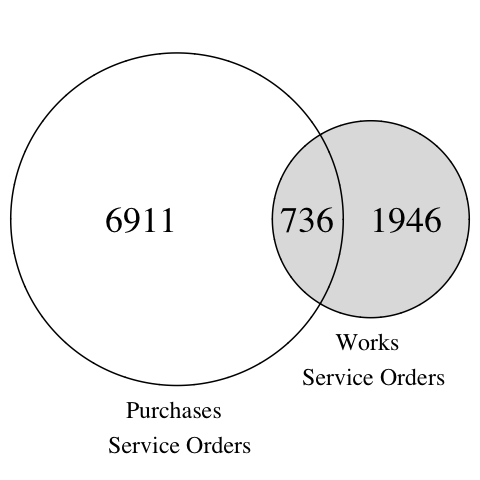
\includegraphics[width=0.3\linewidth]{venn}
\end{figure}

As \citet{GrimmerTextDataPromise2013a} rightly point out, no text analysis algorithm is perfect and only relying on keyword matches could potentially lead to misclassification of service orders. Let us suppose that one description reads ``expenditures made in accordance with primary education program.'' Using unigram ``expenditure'' would yield a match for this service order to the purchases group, but in fact auditors might be looking at bonus payments for high-performing teachers. These resources could also be directed for school construction. In the first case, the service order should not be have been included in any group because it does not carry any procurement component. In the second case, it should have also been marked as public works.

We address these classification problems in three ways: (i) using means comparison tests of match quality discussed in \citet{AssumpcaotextfindDataDrivenText2018}; (ii) comparing the performance of the same search patterns on another textual description for a subset of service orders; (iii) finally, comparing the results from the textual classification algorithm to that of procurement violations reported by CGU auditors. We discuss these three tests in turns in the following sections.

\subsection{Means Tests}\label{subsec:quality1}

The first test on match quality is the means comparison test presented in \citet{AssumpcaotextfindDataDrivenText2018}, whose reasoning is simple. Increasing the number of procurement-related terms in the search pattern is not necessarily good practice as we increase the chance of misclassifying service orders as procurement when in fact they are not; words can take on different meanings depending on their contexts, so the more search terms we use the more likely type I error is. Ideally, we would want to use as few \emph{n}-grams as possible while still identifying all possible procurement matches. In order to do this, what \citet{AssumpcaotextfindDataDrivenText2018} suggests is testing match quality by incrementally comparing sample means identified by \emph{n} + 1 vs.~\emph{n} keywords. This method translates into a check on whether the sample identified by one additional keyword is significantly better than the previous sample with one fewer term. The program developed by \citet{AssumpcaotextfindDataDrivenText2018} runs such check and the results are reported in the table below:
% latex table generated in R 3.5.0 by xtable 1.8-2 package
% Thu Jun  7 14:41:26 2018
\begin{table}[!htbp]
  \caption{\label{tab:purchasesresults} Purchases Search Results}
  \centering
  \small
  \begin{tabular}{rrrrrrr}
  \hline

  \hline
  & Total & \multicolumn{4}{c}{Average} & Means \\ \cline{3-6}
  & Finds & Find & Length & Position & TF-IDF & test p-value \\
  \hline
  ``aquisi'' & 3716 & 1.052 & 27.757 & 4.649 & 0.084 & . \\
  ``execu'' & 2261 & 1.190 & 47.662 & 13.173 & 0.075 & 0.000 \\
  ``equipame'' & 1117 & 1.005 & 60.645 & 39.853 & 0.168 & 0.000 \\
  ``ve{[}íi{]}culo'' & 717 & 0.713 & 38.969 & 11.948 & 0.094 & 0.000 \\
  ``despesa'' & 667 & 1.006 & 40.856 & 19.474 & 0.110 & 0.000 \\
  ``aplica{[}çc{]}'' & 604 & 0.846 & 24.603 & 11.389 & 0.135 & 0.000 \\
  ``medicamento(.)*peaf'' & 570 & 3.367 & 13.167 & . & 0.794 & 0.000 \\
  ``compra'' & 449 & 1.002 & 5.178 & 2.323 & 2.305 & 0.000 \\
  ``recurso(.)*financ'' & 425 & 1.599 & 33.416 & . & 0.183 & 0.000 \\
  ``unidade(.)*m{[}óo{]}ve(.)*sa{[}úu{]}de'' & 364 & 0.897 & 9.365 & . & 0.384 & 0.000 \\
  ``pnate'' & 283 & 1.000 & 22.544 & 21.484 & 2.186 & 0.000 \\
  ``transporte(.)*escola'' & 201 & 1.360 & 18.493 & . & 0.411 & 0.000 \\
  ``desenv(.)*ensino'' & 167 & 5.054 & 37.168 & . & 0.658 & 0.000 \\
  ``kit'' & 134 & 1.067 & 7.836 & 3.590 & 1.292 & 0.000 \\
  ``siafi'' & 124 & 1.016 & 18.008 & 7.298 & 1.333 & 0.000 \\
  ``implementa{[}çc{]}'' & 94 & 0.794 & 32.032 & 4.904 & 0.130 & 0.000 \\
  ``adquir'' & 68 & 1.338 & 29.015 & 17.250 & 0.355 & 0.000 \\
  ``pme(.)*2004'' & 67 & 0.727 & 5.657 & . & 1.711 & 0.000 \\
  ``aparelhamento'' & 4 & 1.000 & 11.250 & 2.500 & 0.716 & 0.045 \\ \hline
   Total & 7647 & . & 29.263 & . & . & 0.000 \\
  \hline

  \hline
  \end{tabular}
\end{table}


The search terms are sorted in descending order by the number of service orders they identify (column 1). Column 6 displays \emph{p}-values for means tests across samples, where each mean is the sum of observations found by \emph{any} of the search items before, and inclusive of, any particular row over the total number of observations.\footnote{This is also known as an alternative search where all search conditions are connected by an ``or'' statement.} For example, the p-value in row 3 tells us that including search word ``equipame'' to the pattern ``aquisi'' or ``execu'' identifies a significantly different, and in this case, larger sample at the 1\% level.

The works sample is a third of the size of the purchases group and two of its search items do not significantly identify a new sample (``saneamento'' and ``conclus{[}ãa{]}o''). Despite having positive individual finds reported in column 1, table \ref{tab:worksresults}, the means test in column 6 suggests that these finds are not new service orders in addition to what had already been identified by the the previous search terms.\footnote{The search without these terms (available upon request) yields 2,679 service orders, just three short of the total in table \ref{tab:worksresults}. Nevertheless, we keep the two items in the search algorithm for additional tests discussed in section \ref{subsec:quality2}.}
% latex table generated in R 3.5.0 by xtable 1.8-2 package
% Thu Jun  7 14:41:31 2018
\begin{table}[!htbp]
\centering
\caption{Works Search Results} 
\label{taba3}
\begin{tabular}{rrrrrrr}
  \hline
 & Total Finds & Average Find & Average Length & Average Position & Average TF-IDF & Means test p-value \\ 
  \hline
1 & 954 & 0.597 & 21.822 & 4.283 & 0.153 & . \\ 
  2 & 877 & 1.003 & 12.754 & 7.023 & 1.658 & 0.000 \\ 
  3 & 767 & 1.021 & 50.811 & 4.001 & 0.074 & 0.000 \\ 
  4 & 614 & 0.859 & 88.894 & 22.000 & 0.055 & 0.000 \\ 
  5 & 366 & 1.000 & 39.109 & 6.615 & 0.144 & 0.000 \\ 
  6 & 333 & 0.996 & 31.156 & . & 0.175 & 0.000 \\ 
  7 & 307 & 1.029 & 14.704 & 6.316 & 0.429 & 0.000 \\ 
  8 & 279 & 1.360 & 38.315 & . & 0.128 & 0.000 \\ 
  9 & 255 & 1.024 & 37.035 & 31.412 & 0.187 & 0.000 \\ 
  10 & 170 & 0.303 & 48.871 & 20.253 & 0.031 & 0.045 \\ 
  11 & 541 & 0.626 & 29.115 & 9.839 & 0.141 & 0.000 \\ 
  12 & 58 & 1.000 & 47.017 & 14.190 & 0.135 & 0.025 \\ 
  13 & 35 & 0.769 & 33.257 & 19.029 & 0.141 & 0.000 \\ 
  14 & 24 & 1.000 & 38.000 & 23.083 & 0.755 & 0.317 \\ 
  15 & 21 & 4.455 & 62.619 & . & 0.429 & 0.045 \\ 
  16 & 4 & 0.750 & 25.750 & 8.000 & 0.276 & 0.157 \\ 
  17 & 2682 & . & 34.882 & . & . & 0.000 \\ 
   \hline
\end{tabular}
\end{table}


Means tests are important to map out the relationship between search items, both within and across groups, but they do not tell us anything about the relationship between search items and their latent procurement groups. In other words, the search terms might be picking up groups that are internally consistent but that do not map onto the procurement types in Law 8,666/93. In sections \ref{subsec:quality2} and \ref{subsec:quality3}, we test if these search patterns really reflect the procurement legislation in Brazil.

\subsection{Textual Descriptions}\label{subsec:quality2}

CGU service orders can best be described as investigations on the use of
public resources transferred from the federal government to Brazilian
municipalities. There are six transfer types and each service order
investigates only one type at a time. Since the procurement categories
set out in Law 8,666/93 apply to all public procurements at all
government levels, transfer types are irrelevant for constructing our
discretion measure. Nonetheless, we can test the quality of our classification algorithm on one type of these transfers.

Federal grants (\emph{convênios} in Portuguese) are narrow transfer
agreements signed by the federal government, its agencies, states and
municipalities for the delivery of governmental programs. They are
voluntary, time-limited transfers implementing policies at the local
level, such as vaccinations and the construction of community health
clinics. The most important feature of these grants, however, is that
each of them also has an individual textual description of its purpose,
e.g.~a tractor purchase for a rural community in a given municipality.
Thus, for a subset of service orders that are investigations of the use
of grants in Brazilian municipalities, we have two
different textual descriptions of resource use: CGU's, from their audit
report, and the federal government's, available online at the
Transparency Portal.\footnote{\url{http://www.portaltransparencia.gov.br/}}
% latex table generated in R 3.5.0 by xtable 1.8-2 package
% Thu Jun  7 16:23:00 2018
\begin{table}[!htbp]
\centering
\caption{Classification by Textual Description} 
\label{taba4}
\begin{tabular}{rr}
  \hline
0 & 1 \\ 
  \hline
115 & 144 \\ 
   83 & 1473 \\ 
  1546 & 269 \\ 
  404 & 1649 \\ 
   \hline
\end{tabular}
\end{table}


There is a total of 3,868 service orders for which we have descriptions both from CGU and from the federal government. In table \ref{tab:textualdescription}, we report the results of the search algorithm both in the service order (row-wise) and the transfer (column-wise) descriptions. We evaluate the performance of the search algorithm by checking whether it assigns the same service order to the same procurement group \emph{regardless of the description in which it searches for the key terms}. In other words, the smaller the number of times that the algorithm assigns any service order to a different group when it switches to another textual description, the better. The diagonal (\emph{Yes-No; No-Yes}) should be populated by only a small number of transfers compared to the overall sample.

This is a particularly important point for the classification method proposed here. The means test conducted in section \ref{subsec:quality1} provides internal consistency because it compares and checks whether more observations are matched when more search terms are included; the tabulation across descriptions here provides external consistency because it compares and checks if the classification algorithm is independent of search target (description). It resembles a false positive (type I error) test because we can roughly calculate the percentage of misclassification of service orders. In panel A, the service order description search assigns 1,556 to the purchases group, out of which 83 were not simultaneously assigned to the same group in the grant description search, yielding a 5.3\% false positive rate. In panel B, the service order search marks 2,053 observations to the works group, where 404 are not simultaneously marked when the search is performed in the grant description (a 19.7\% type I error rate).\footnote{The inverse misclassification rates are also reassuring: false positives are 8.9\% and 14.0\% for purchases and works respectively when we first classify observations using grant descriptions and then move on to service order descriptions.}

\subsection{Procurement Violations}\label{subsec:quality3}

Though section \ref{subsec:quality2} supports external validity by showing that the service order classification is consistent across textual descriptions, we run the last robustness check here using the actual procurement violations reported by CGU.

The findings reported by auditors are coded into 35 infractions of the use of public resources, nine of which violations of procurement rules and one violation of public works rules. Thus, we know with certainty that service orders for which there are any of the nine procurement violations (ten if public works) are in fact procurement-related and should be classified either as purchases, works, or both. As opposed to section \ref{subsec:quality2}, this resembles a false negative (type II error) test on yet another subset of observations for which certain infractions were reported.\footnote{The reason why this is a type II error test, instead of type I, resides on the way the test samples are defined. In section \ref{subsec:quality2}, both sample assignments (by matching procurement keywords in the service order or grant description) can be the ``correct'' procurement sample against which the match on the alternative description might yield false positives. In this section, we know with certainty that the sample identified by procurement infractions is in fact the correctly identified sample, since there cannot exist a procurement violation where no procurement has occurred. It makes the unidentified observations false negatives because they should have been classified as procurement-related service orders. This sample is clearly underidentified, as there are many procurement-related service orders that simply followed Law 8,666/93 and thus carry no infraction, but still, within this subset of all CGU investigations, it provides us with a good counterfactual against which to test our classification mechanism.}
\begin{table}[!htbp]
  \caption{\label{tab:textbycode}Classification by SO Text and Procurement Code}
  \centering
  \scriptsize
  \begin{tabular}{cr|rrr}
    \hline

    \hline
    \multicolumn{5}{c}{\emph{Panel A: Purchases Group}} \T \B \\
    \hline
    & & \multicolumn{3}{c}{Procurement Code} \T \B \\
    & & No  & Yes  & Total \T \B \\
    \hline
    \multirow[c]{4}{*}{\begin{sideways}SO\end{sideways}} & No & 2487 & 319 & 2806  \T \B \\
    & Yes   & 6137 & 3456 & 9593  \T \B \\
    & Total & 8624 & 3775 & 12399 \T \B \\
    \hline

    \hline
  \end{tabular} \hspace{6pt} \begin{tabular}{cr|rrr}
    \hline

    \hline
    \multicolumn{5}{c}{\emph{Panel B: Works Group}} \T \B \\
    \hline
    & & \multicolumn{3}{c}{Procurement Code} \T \B \\
    & & No  & Yes  & Total \T \B \\
    \hline
    \multirow[c]{4}{*}{\begin{sideways}SO\end{sideways}} & No & 2462 & 344 & 2806  \T \B \\
    & Yes   & 5791 & 3802 & 9593  \T \B \\
    & Total & 8253 & 4146 & 12399 \T \B \\
    \hline

    \hline
  \end{tabular}
\end{table}

The total number of service orders with at least one procurement infraction is 3,775 (4,146 if we include the public works infraction), which is the sum of column 2 in table \ref{tab:textbycode}, panels A and B. The false negative rate is 8.5\% and 9.9\%, respectively, for purchases-only and works procurements. This means that 319 and 344 service orders should have been classified as procurement by our textual search algorithm but were not.

Although no text analysis mechanism is perfect, the evidence presented here supports our choice of classification algorithm. The identification of procurement orders is internally consistent (section \ref{subsec:quality1}), there are very few incorrect assignments of service orders to procurement (section \ref{subsec:quality2}), and the sample which was identified as procurement maps well onto the latent types in the Brazilian procurement legislation (section \ref{subsec:quality3}).
\newpage

\section{CEPESP Coding of Service Orders}\label{sec:appendixB}

\begin{table}[!htbp]
  \caption{\label{tab:codes} Infraction Classification}
  \centering
  \scriptsize
  \begin{tabular}{r|l}
  \hline

  \hline
  Code \#& Code Description \\
  \hline
  \multicolumn{2}{r}{Bottom-up Monitoring} \\
  \hline
   (01) & Citizen's committee has not been properly set up. \\
   (02) & Committee does not monitor programs. \\
   (03) & Committee has poor working conditions. \\
  \hline
  \multicolumn{2}{r}{Human Resources} \\
  \hline
   (24) & Officials did not meet their assigned workload. \\
   (27) & Officials received insufficient training. \\
   (28) & Officials were not properly hired. \\
   (32) & Officials received incorrect wage or benefit payment. \\
  \hline
  \multicolumn{2}{r}{Infrastructure} \\
  \hline
   (20) & Physical infrastructure is inappropriate for program implementation. \\
   (21) & Shortage of government goods/supplies. \\
   (22) & Poor stock management of government goods. \\
   (26) & Government goods/supplies were inadequately labeled. \\
   (29) & Government goods/supplies were poorly preserved. \\
  \hline
  \multicolumn{2}{r}{Performance} \\
  \hline
   (15) & Payments shifted to other government needs. \\
   (17) & Municipality did not supplement program funding. \\
   (18) & Program has not been entirely implemented or its goals were only partially met. \\
   (19) & Public works have not followed construction rules. \\
   (23) & Poor service provided to citizens. \\
   (25) & Program documentation was wrong. \\
   (33) & Idle funds were not transfered to savings/money market accounts. \\
   (34) & Program participants did not receive their benefits. \\
   (35) & Beneficiaries did not meet conditions for inclusion in program. \\
   (36) & Poor beneficiary data management. \\
  \hline
  \multicolumn{2}{r}{Procurement} \\
  \hline
  *(04) & Public tender was not publicized. \\
  *(05) & Tender winner presented forged price estimates. \\
  *(06) & Shell companies have participated in tender. \\
   (07) & Tender documentation was wrong. \\
  *(08) & Tender documentation was forged. \\
  *(09) & Tender participant received special treatment. \\
   (10) & Multiple (non-corruption) tender problems. \\
  *(30) & Wrong category was applied. \\
  *(31) & Tender was incorrectly dismissed. \\
  \hline
  \multicolumn{2}{r}{Private Appropriation} \\
  \hline
  *(11) & Good/service was overpriced. \\
  *(12) & Supplier used forged receipts to claim payments. \\
  *(13) & Payments were unaccompanied by receipts. \\
  *(14) & Payments made to parties unrelated to policy implementation. \\
  \hline
  \multicolumn{2}{r}{Ungrouped} \\
  \hline
  (00, 98, 99) & No infractions were found. \\
  \hline

  \hline
  \multicolumn{2}{l}{*Corruption infractions.}
  \end{tabular}
\end{table}

\newpage

\section{Service Amount Manipulation}\label{sec:appendixC}

The identification strategy in this paper relies on the assumption that municipal officials do not (completely) manipulate public expenditure amounts in order to avoid stricter procurement rules. In other words, the public procurement processes carried out just below and above any of the three discretion thresholds, which are uniquely determined by procurement amount, are equal except for the rules set out in Law 8,666/93 -- thus they are good counterfactuals for testing the effect of expenditure discretion on performance. We present below the \citet{McCraryManipulationrunningvariable2008} test for manipulation of the running variable for all six cutoffs in the Brazilian procurement legislation, which show no significant difference between service order density just below and above five of the six discretion cutoffs imposed by Law 8,666/93. The only discontinuity for which variables do not seem comparable is purchases cutoff 3, which we drop from the analysis in sections \ref{sec:methodology} and \ref{sec:result}.

\begin{figure}[!htbp] \centering
  \caption{\label{fig:manipulationtests} Manipulation Tests at SO Cutoff Amounts}
  \begin{tabular}{cc}
  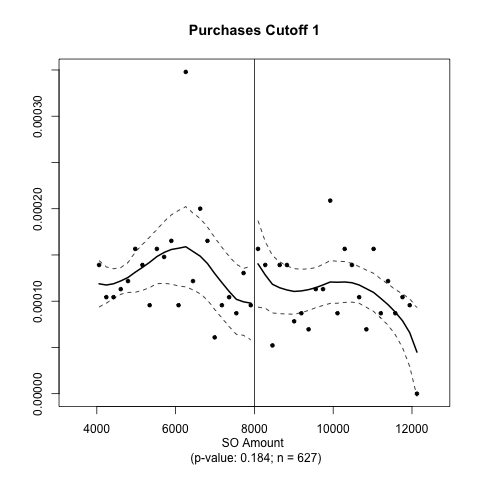
\includegraphics[scale=.24]{purchasesmanipulation1} & 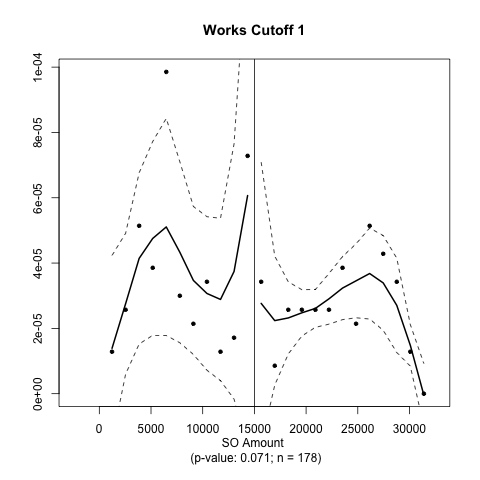
\includegraphics[scale=.24]{worksmanipulation1} \\
  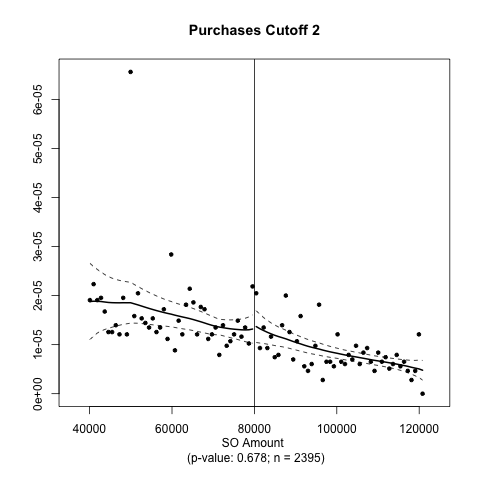
\includegraphics[scale=.24]{purchasesmanipulation2} & 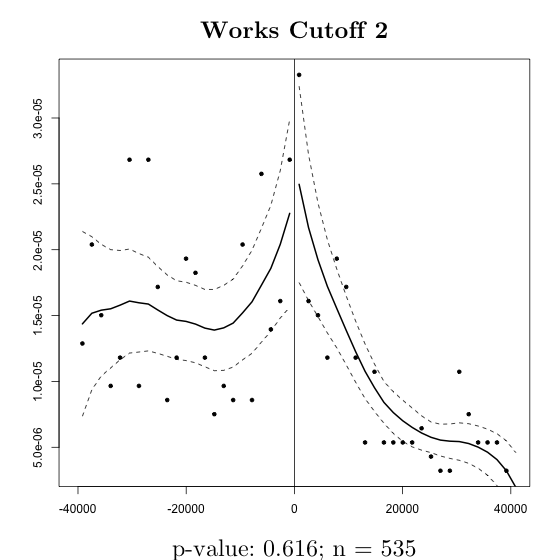
\includegraphics[scale=.24]{worksmanipulation2} \\
  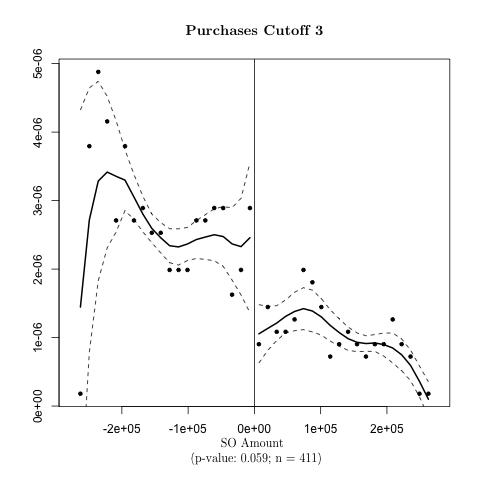
\includegraphics[scale=.24]{purchasesmanipulation3} & 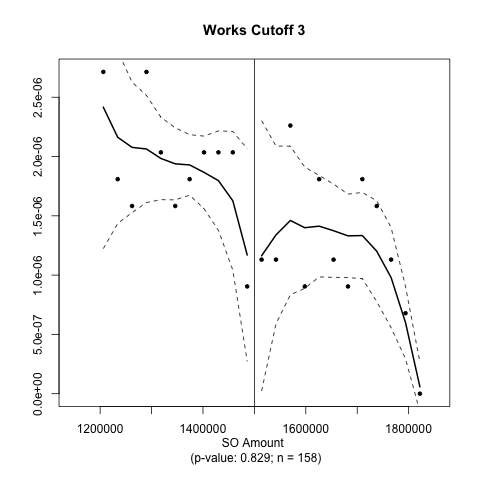
\includegraphics[scale=.24]{worksmanipulation3} \\
  \end{tabular}
\end{figure}

\end{document}